\documentclass[compress, handout]{beamer}

\usepackage{beamerthemesplit}
\usepackage{algorithm}
\usepackage{algorithmic}
\usepackage{amsmath}
\usepackage{amssymb}
\usepackage{amsfonts}
\usepackage{multimedia}
\usepackage{hyperref}
\usepackage{pgf}
\usepackage{subfigure}
\usepackage{array}
\usepackage{color}

% Definitions for our custom syntax stuff.
\usepackage{mydefs}

\hyphenation{mutual illuminations}
\setbeamersize{text margin left=0.3cm, text margin right=0.3cm}
\usetheme{Frankfurt}

%\usepackage{ifthen}
%\newboolean{includethis}
%\setboolean{includethis}{false}
%\newcommand{\ifinclude}[1]{\ifthenelse{\boolean{includethis}}{#1}{}}

%\ifinclude{
%\begin{frame}{Slide title}
%this slide will be hidden
%\end{frame}
%}

\title[Robust and Scalable Face Recognition]{Robust and Scalable Face Recognition via Sparse Representation and Parallel Programming}
\author{Andrew Wagner} 
\institute{Department of Electrical and Computer Engineering\\
University of Illinois at Urbana-Champaign\\
}
\date{May 4, 2009}

%\logo{\includegraphics[width=0.5in]{figures/pdl_logo}}

%\includeonlyframes{current}

\begin{document}

\frame{\titlepage}

%%%%%%%%%%%%%%%%%%%%%%%%%%%%
\frame{\tableofcontents}

\section{Introduction}

\subsection{Introduction}
\frame{
\frametitle{Why is face recognition a good way to recognize people?}
\begin{itemize}
\item Non-contact
\item Potentially faster than gait or voice recognition
\item No special hardware needed for recognition (unlike Iris recognition)
\item Attacks would probably be obvious to bystanders
\item Recognized person need not do anything
\end{itemize}
}



\frame{
\frametitle{Importance for humans}
\begin{itemize}
\item 
Humans seem to have evolved domain specific ``wetware'' for recognizing faces, called the fusiform face area.  \footnote{"Early (M170) activation of face-specific cortex by face-like objects", Hadjikhani N, et al., Feb 2009, Neuroreport 20: 403.}
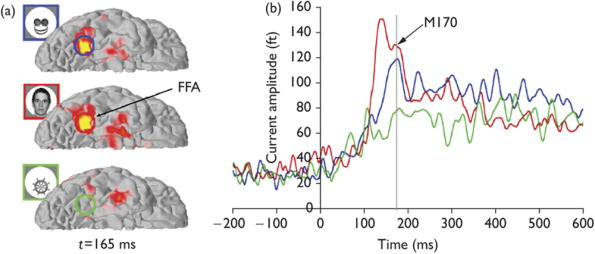
\includegraphics[width=0.9\textwidth]{images/fusiform_face_area.jpg}
\item Face Blindness (Prosopagnosia) congenital in 2.5\% of population \\
%\item Capgras syndrome
\end{itemize}
}


%!TEX root = prelim.tex



%\frame{
%\frametitle{Why is face recognition a good way to recognize people?}
%\begin{itemize}
%\item Non-contact
%\item Potentially faster than gait or voice recognition
%\item No special hardware needed for recognition (unlike Iris recognition)
%\item Attacks would probably be obvious to bystanders
%\item Recognized person need not do anything
%\end{itemize}
%}

%\frame{
%\frametitle{Importance for humans}
%\begin{itemize}
%\item 
%Humans seem to have evolved domain specific "wetware" for recognizing faces, called the fusiform face area.  \footnote{"Early (M170) activation of face-specific cortex by face-like objects", Hadjikhani N, et al., Feb 2009, Neuroreport 20: 403.}
%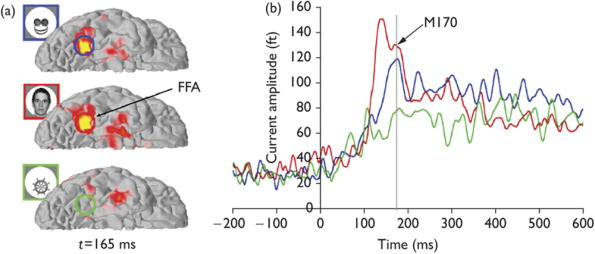
\includegraphics[width=0.9\textwidth]{images/fusiform_face_area.jpg}
%\item Face Blindness (Prosopagnosia) congenital in 2.5\% of population \\
%%\item Capgras syndrome
%\end{itemize}
%}

%\subsection{Review of Problem}
\frame{
\frametitle{Status of image based face recognition in industry}
\begin{itemize}
\item Barely works for entertainment purposes with a small number of users.
\begin{itemize}
\item iPhoto
\item Picassa
\item Windows Live Photo Gallery (Beta)
\end{itemize}
\item A failure for security applications
\begin{itemize}
\item High profile trial at Boston Logan Airport failed over half of the time.
\item Toshiba laptop face recognition can be broken by holding up a picture
\end{itemize}
\end{itemize}
}

%DREW: PICTURES

\frame{
\frametitle{Status of image based face recognition in academia}
\begin{itemize}
\item Classical algorithms, such as Eigenfaces, LDA, Nearest Neighbor, and Nearest Subspace perform poorly when confronted with test images taken outside of the lab.
\item Three factors dramatically affect the appearance of a face:
\begin{enumerate}
\item Illumination Variation: The appearance of the face depends very strongly on the illumination
\item Alignment Variation: The image depends on the orientation between the camera and subject 
\item Occlusion: Often parts of the face image are covered by other objects
\end{enumerate}
\end{itemize}
}


\frame{
\frametitle{A promising recent direction in face recognition research}
\begin{center}
\vspace{-.2in}
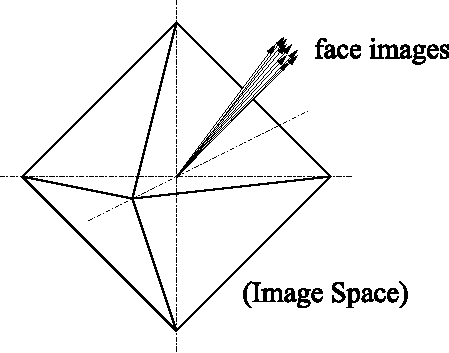
\includegraphics[width=.3\textwidth]{images/bouqet.pdf}\\
\vspace{-.2in}
\end{center}
\begin{itemize}
\item One very promising direction in face recognition research,
{\bf Sparse Representation based Classification (SRC)} [Wright et.\ al. PAMI 2009], achieved state-of-the-art results on Extended Yale B and AR databases.
\item This is a solid foundation, but it is incomplete:
	\begin{itemize}
	\item Assumed perfectly aligned images
	\item Assumed a sufficient number of training illuminations taken under different illuminations
\end{itemize}
\end{itemize}
}



\frame{
\frametitle{The Goal of the Proposed Research}
{\large The goal of my research is to build a complete and scalable face recognition system that can handle  {\bf illumination variation, alignment error, and realistic occlusions.}}\\
\vspace{.2in}
This will entail the following major contributions:
\begin{itemize}
\item Determine what {\bf training illuminations} are sufficient and build an {\bf acquisition system} capable of capturing them
\item Design algorithm for {\bf automatically aligning} test images to training images
\item Improve performance on {\bf contiguous occlusions}
\end{itemize}
}

\frame{\tableofcontents}

%%%%%%%%%%%%%%%%%%%%%%%%%%%%
%\section{Robust Face Recognition}

\section{Illumination}
\frame{\tableofcontents[currentsection, currentsubsection]}
\subsection{Illumination Model}

%!TEX root = prelim.tex

\frame{\frametitle{Compound Effect of Alignment and Illumination}
\renewcommand{\imagesizestring}{height}
\renewcommand{\imagesizea}{0.25\textheight}
\renewcommand{\imagesizeb}{0.15\textheight}
\renewcommand{\gapsizea}{-0mm}
\begin{tabular}[b]{cc@{}b{.5\textwidth}}
% Example for setting the heights of the images
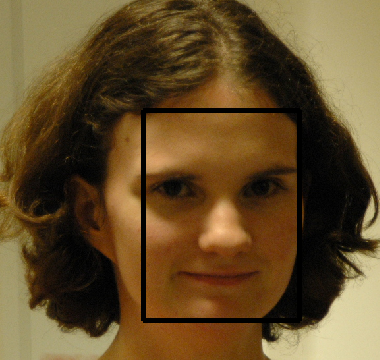
\includegraphics[\imagesizestring=\imagesizea]{figures_cvpr/promo/case1/detector.png}& \hspace{\gapsizea}
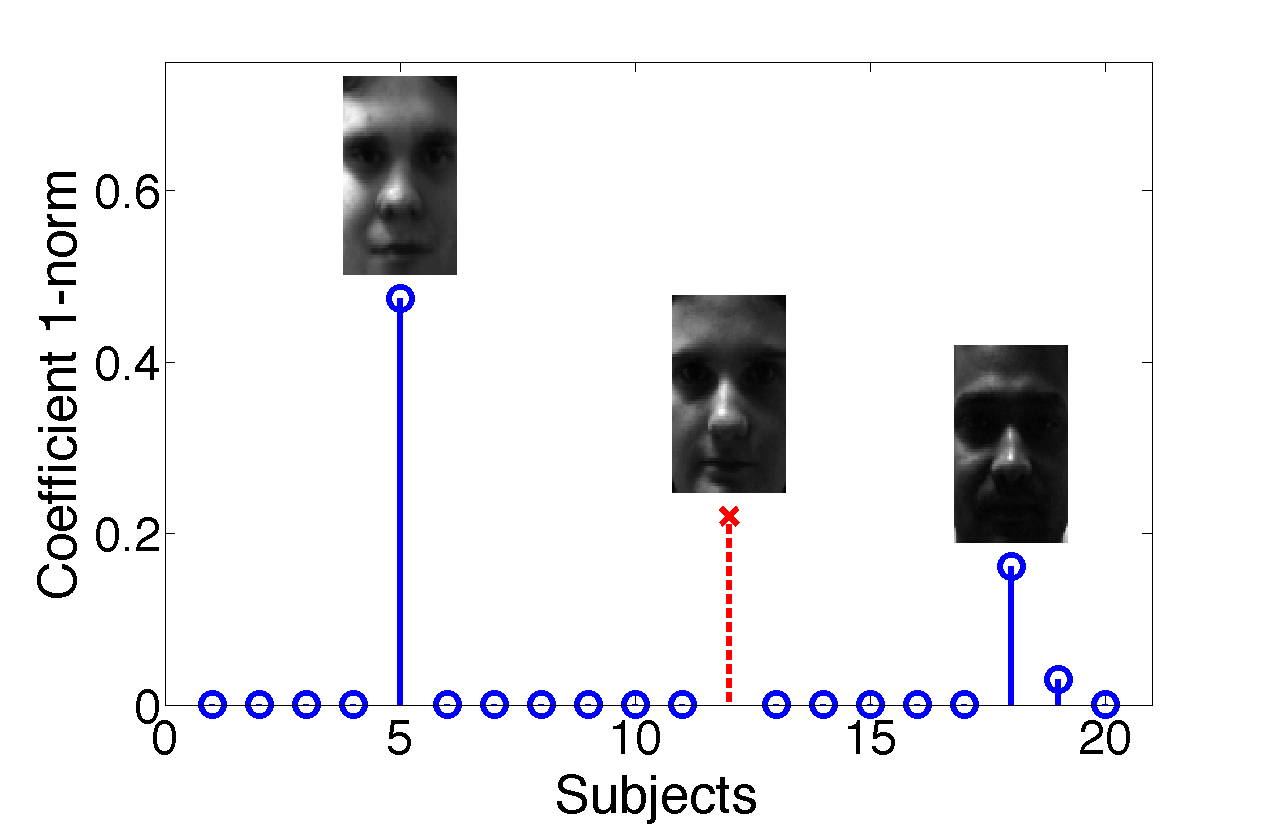
\includegraphics[\imagesizestring=\imagesizea]{figures_cvpr/promo/case1/sci_with_axis_face_case1.png} & 
Poor alignment, {\bf Sufficient training illuminations} \vfill\\
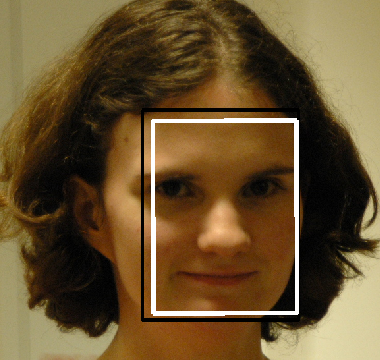
\includegraphics[\imagesizestring=\imagesizea]{figures_cvpr/promo/alignment_and_detector.png}& \hspace{\gapsizea}
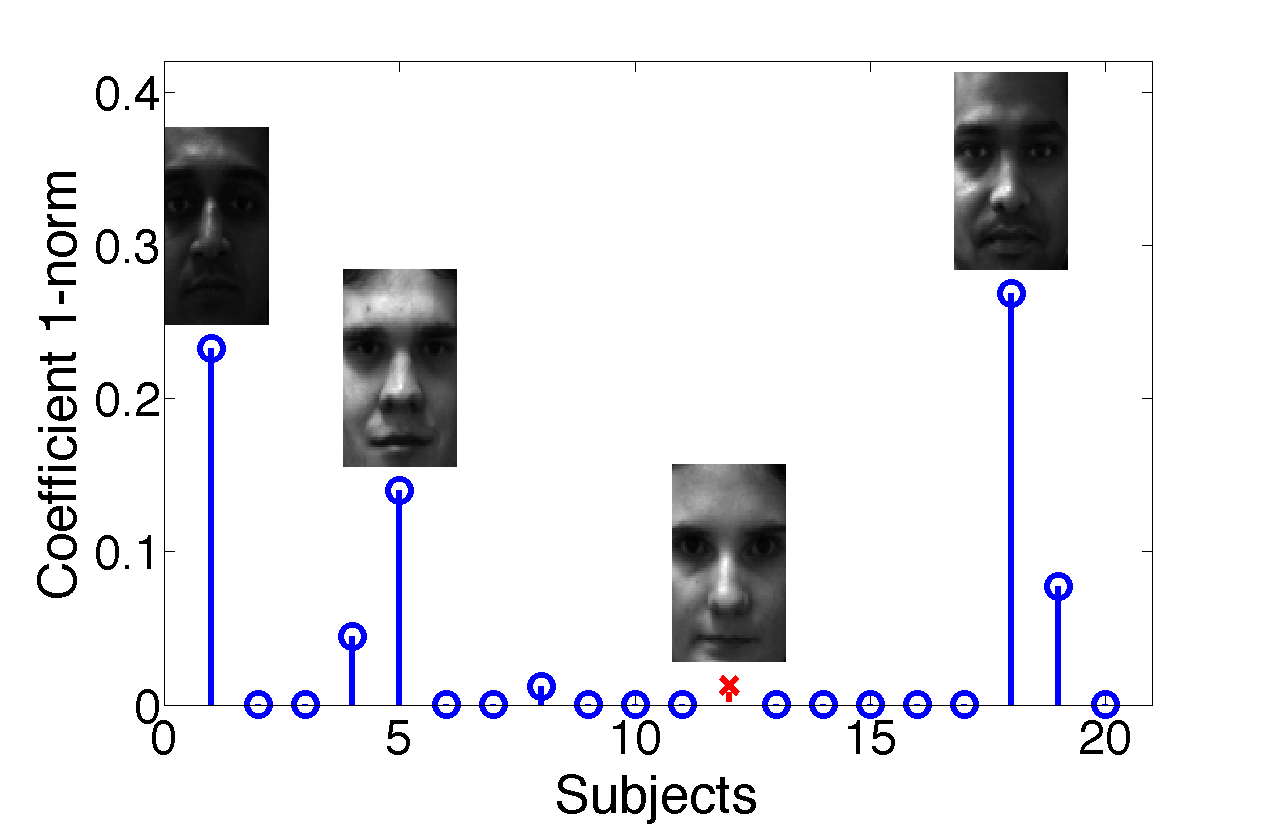
\includegraphics[\imagesizestring=\imagesizea]{figures_cvpr/promo/case2/sci_with_axis_face_case2.png} & 
{Good alignment, {\bf Insufficient training illuminations}}\vfill\\
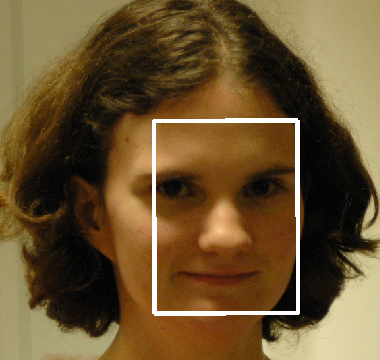
\includegraphics[\imagesizestring=\imagesizea]{figures_cvpr/promo/case3/alignment.png} & \hspace{\gapsizea}
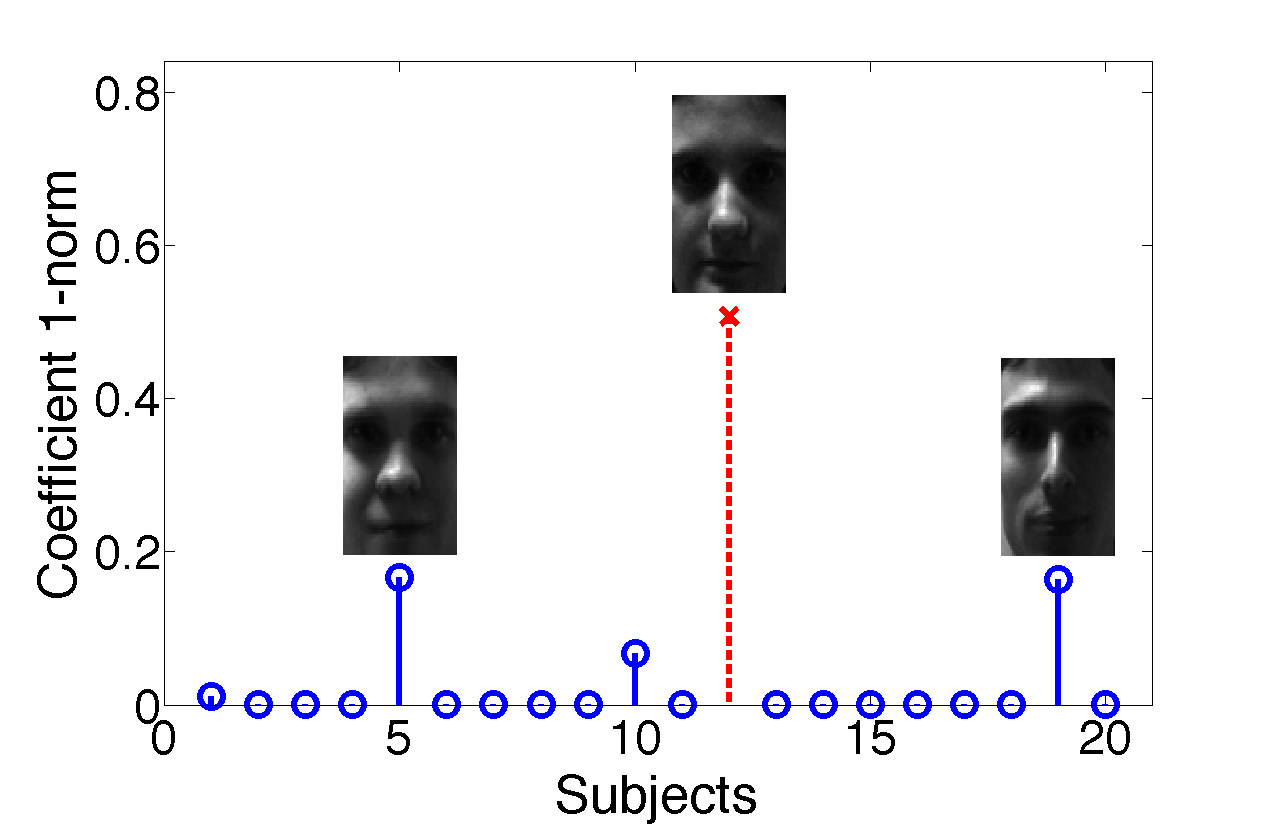
\includegraphics[\imagesizestring=\imagesizea]{figures_cvpr/promo/case3/sci_with_axis_face_case3.png} &
{Good alignment, {\bf Sufficient training illuminations}}\vfill
\end{tabular}
}


\frame{
\frametitle{Linear Illumination Models}
\hspace{.1\textwidth}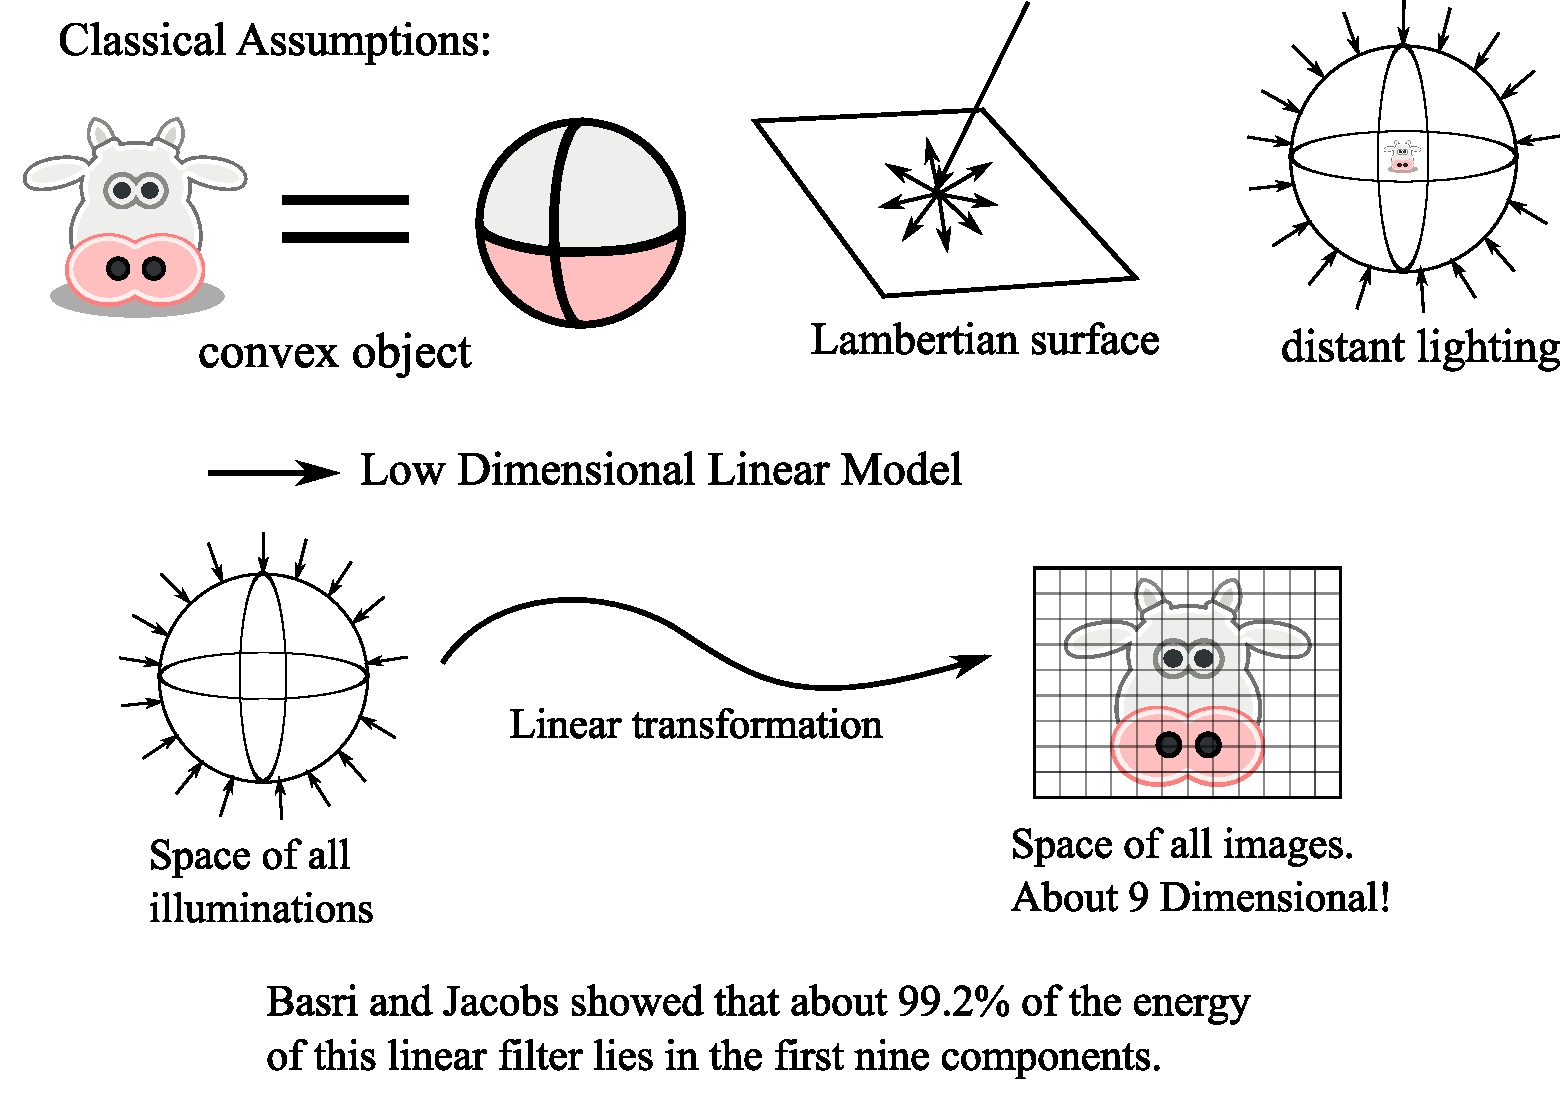
\includegraphics[height=0.8\textheight]{images/linear_illumination_model.pdf}
}

\frame{
\frametitle{Cows are not spherical}
\vspace{-5mm}\begin{center}
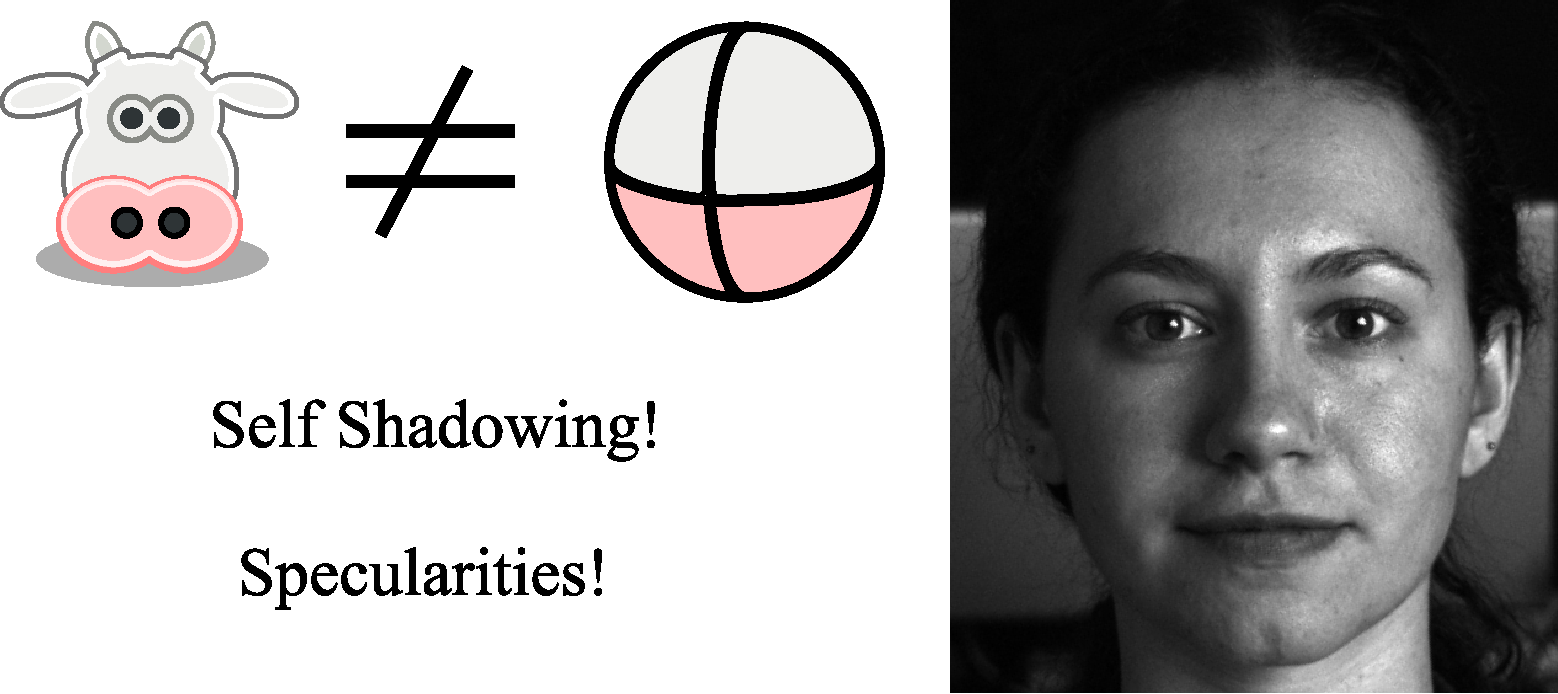
\includegraphics[width=0.9\textwidth]{images/basri4.pdf}
\end{center}\vspace{-5mm}
\begin{itemize}
\item Images still linear WRT illumination
\item {\em Experimentally} determine which training illuminations needed
\end{itemize}
}

%!TEX root = prelim.tex

\subsection{Acquisition System}
\frame{
\frametitle{Training Rig Background}
\begin{columns}

\begin{column}{0.7\textwidth}
Traditional Flash-Based system
\begin{itemize}
\item Used for most public data sets
\item Difficult to reconfigure
\item Does not scale well in the number of flashes
\item Need room sized dome for good angular coverage, distant illumination
\end{itemize}
Projector-Based system
\begin{itemize}
\item Easy to re-configure projector geometry
\item Trivial to change illumination patterns
\item Easier to construct and deploy
\item Very complete angular illumination coverage
\end{itemize}
\end{column}

\begin{column}{0.3\textwidth}
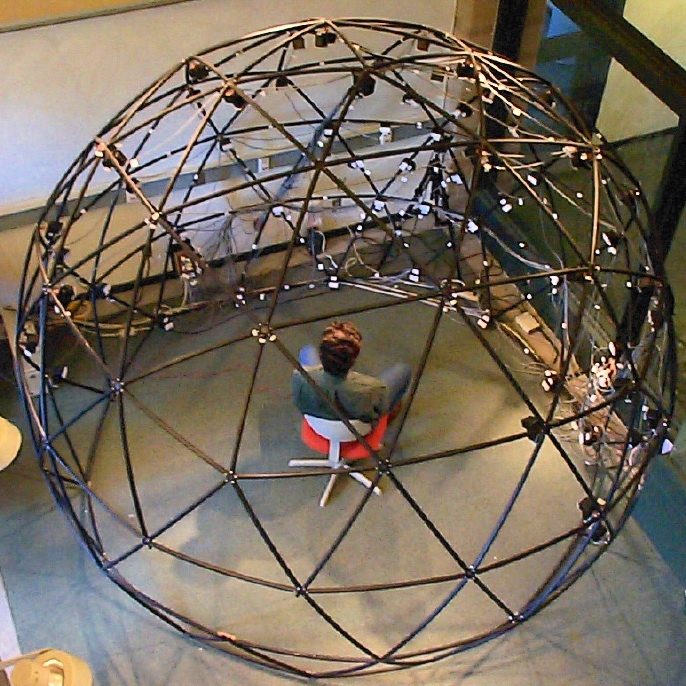
\includegraphics[width=\textwidth]{images/yale_dome.jpg}\\ 
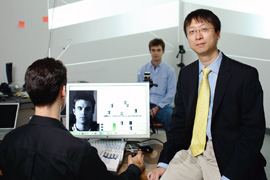
\includegraphics[width=\textwidth]{images/projector_photo.jpg} \\ \vspace{0\textheight}
\end{column}
\end{columns}
}

\frame{
\frametitle{Training Illumination Rig}
\begin{center}
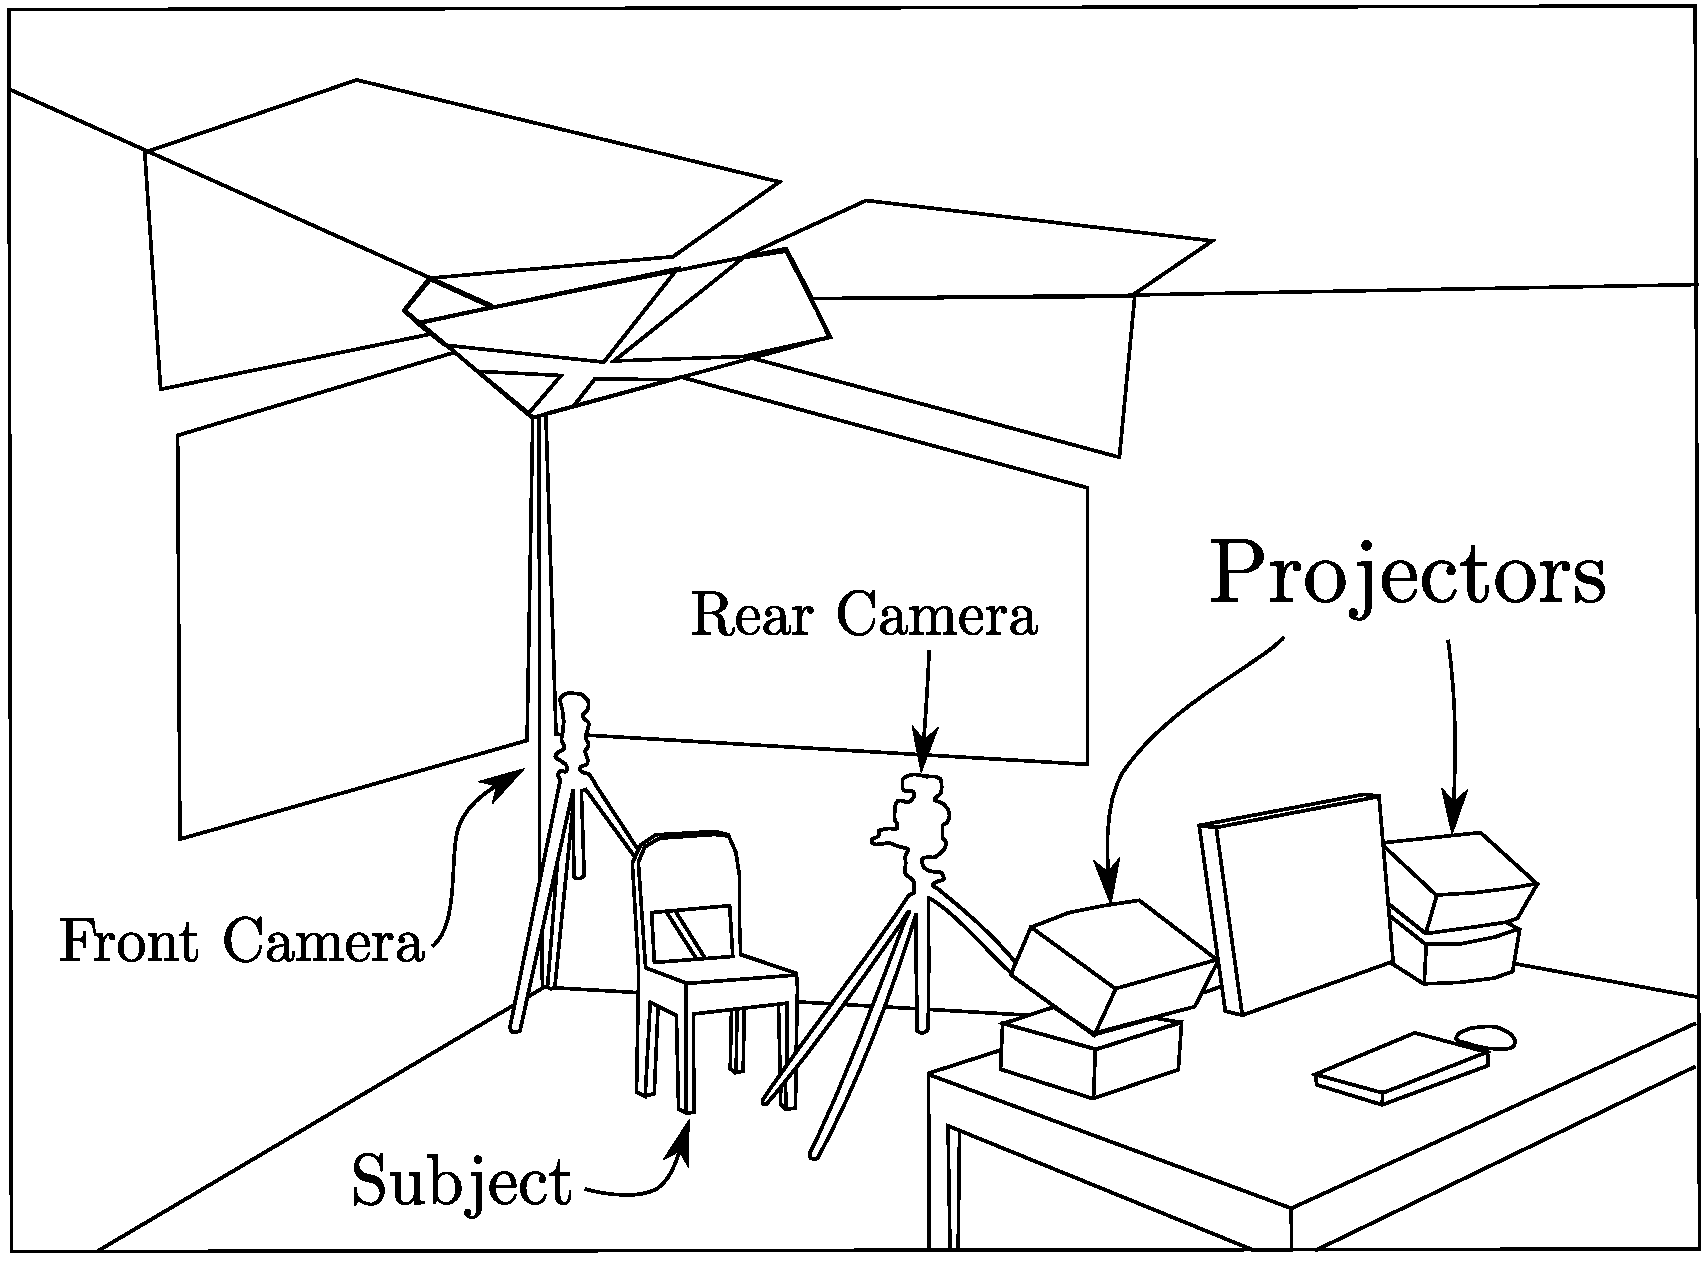
\includegraphics[width=0.8\textwidth]{images/camera_rig_drawings/perspective.pdf}
\end{center}
}

\frame{
\frametitle{Training Illumination Rig}
\begin{columns}
\begin{column}{.5\textwidth}
\begin{center}
Side View\\
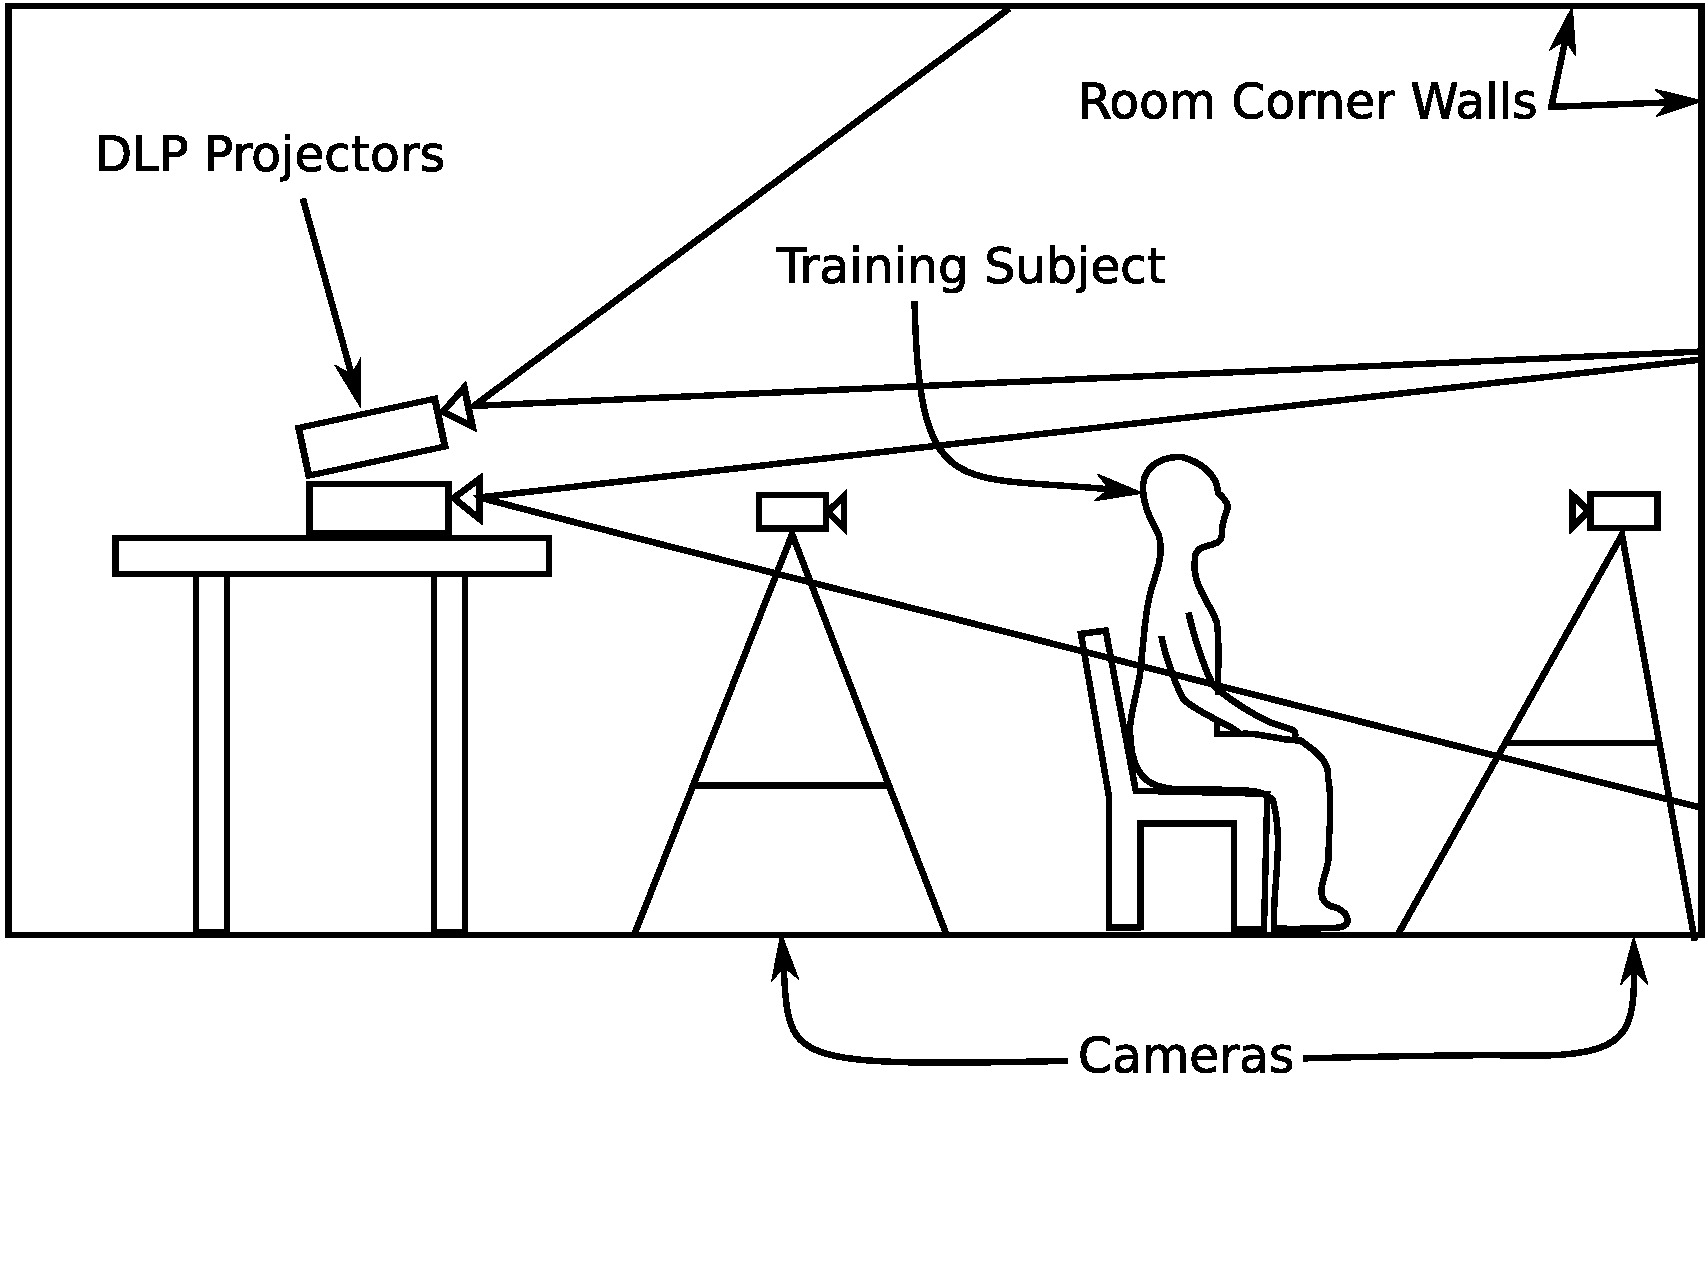
\includegraphics[width=\textwidth]{images/camera_rig_drawings/coverage_side.pdf}
\end{center}
\end{column}
\begin{column}{.5\textwidth}
\begin{center}
Top View\\
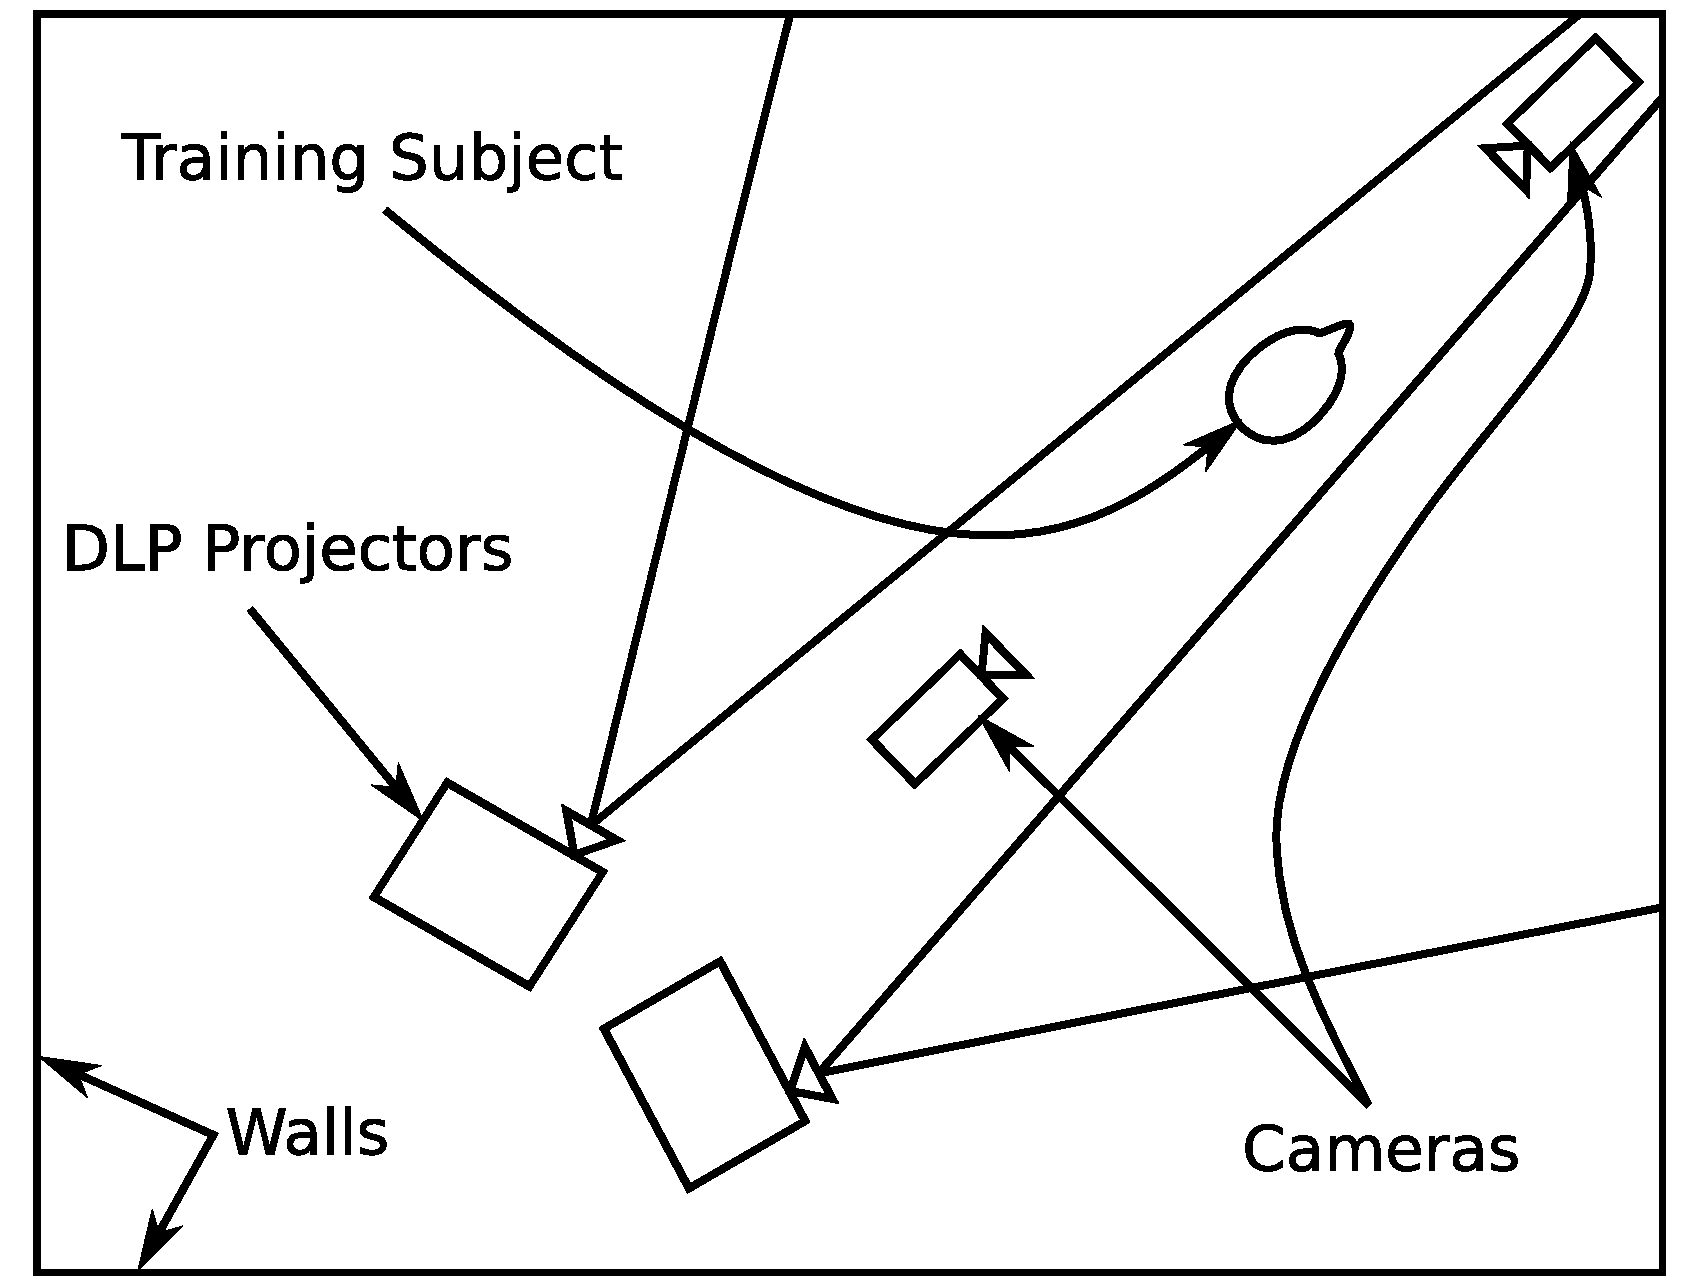
\includegraphics[width=\textwidth]{images/camera_rig_drawings/coverage_top.pdf}
\end{center}
\end{column}
\end{columns}
}

\frame{
\frametitle{So many projector pixels, so little time}
\begin{itemize}
\item Need to narrow down the illumination possibilities.
\item How densely do we need to sample the illumination sphere?
\begin{itemize}
\item Try multiple sets of illuminations
\item Double the resolution in one direction each time
\end{itemize}
\item How much coverage do we need?
\begin{itemize}
\item Try multiple sets of illuminations
\item Gradually increase the coverage radially out from known-important illuminations
\end{itemize}
\end{itemize}
\begin{center}
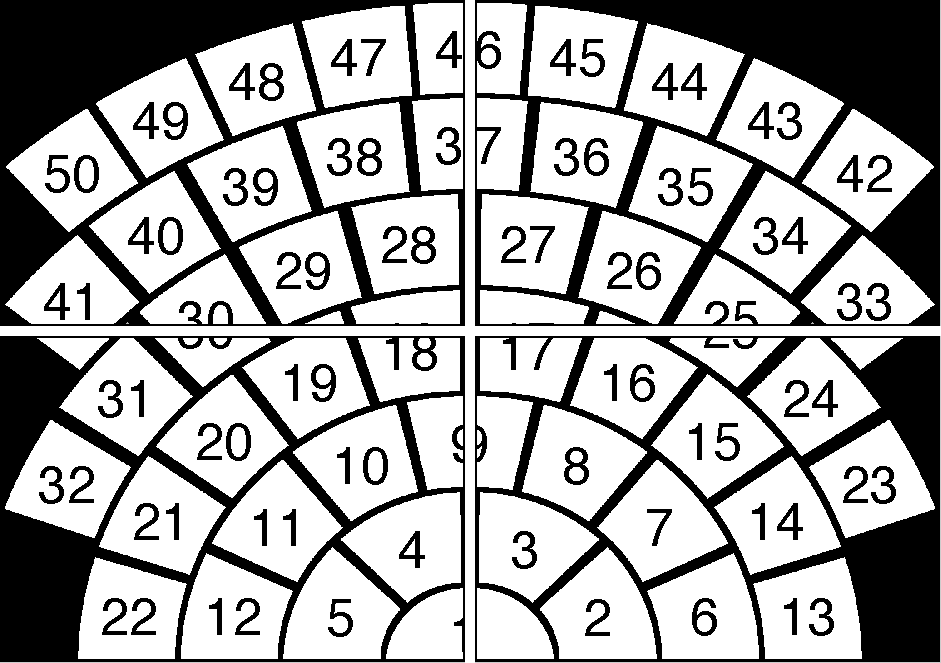
\includegraphics[height=.4\textheight]{figures_cvpr/coverage_experiment_asplode_white.png}
\end{center}
}

\renewcommand{\imagesizestring}{height}
\frame{\frametitle{Illumination Experiment Results}
\renewcommand{\imagesizea}{0.55\textheight}
\begin{center}
\begin{tabular}{cc}
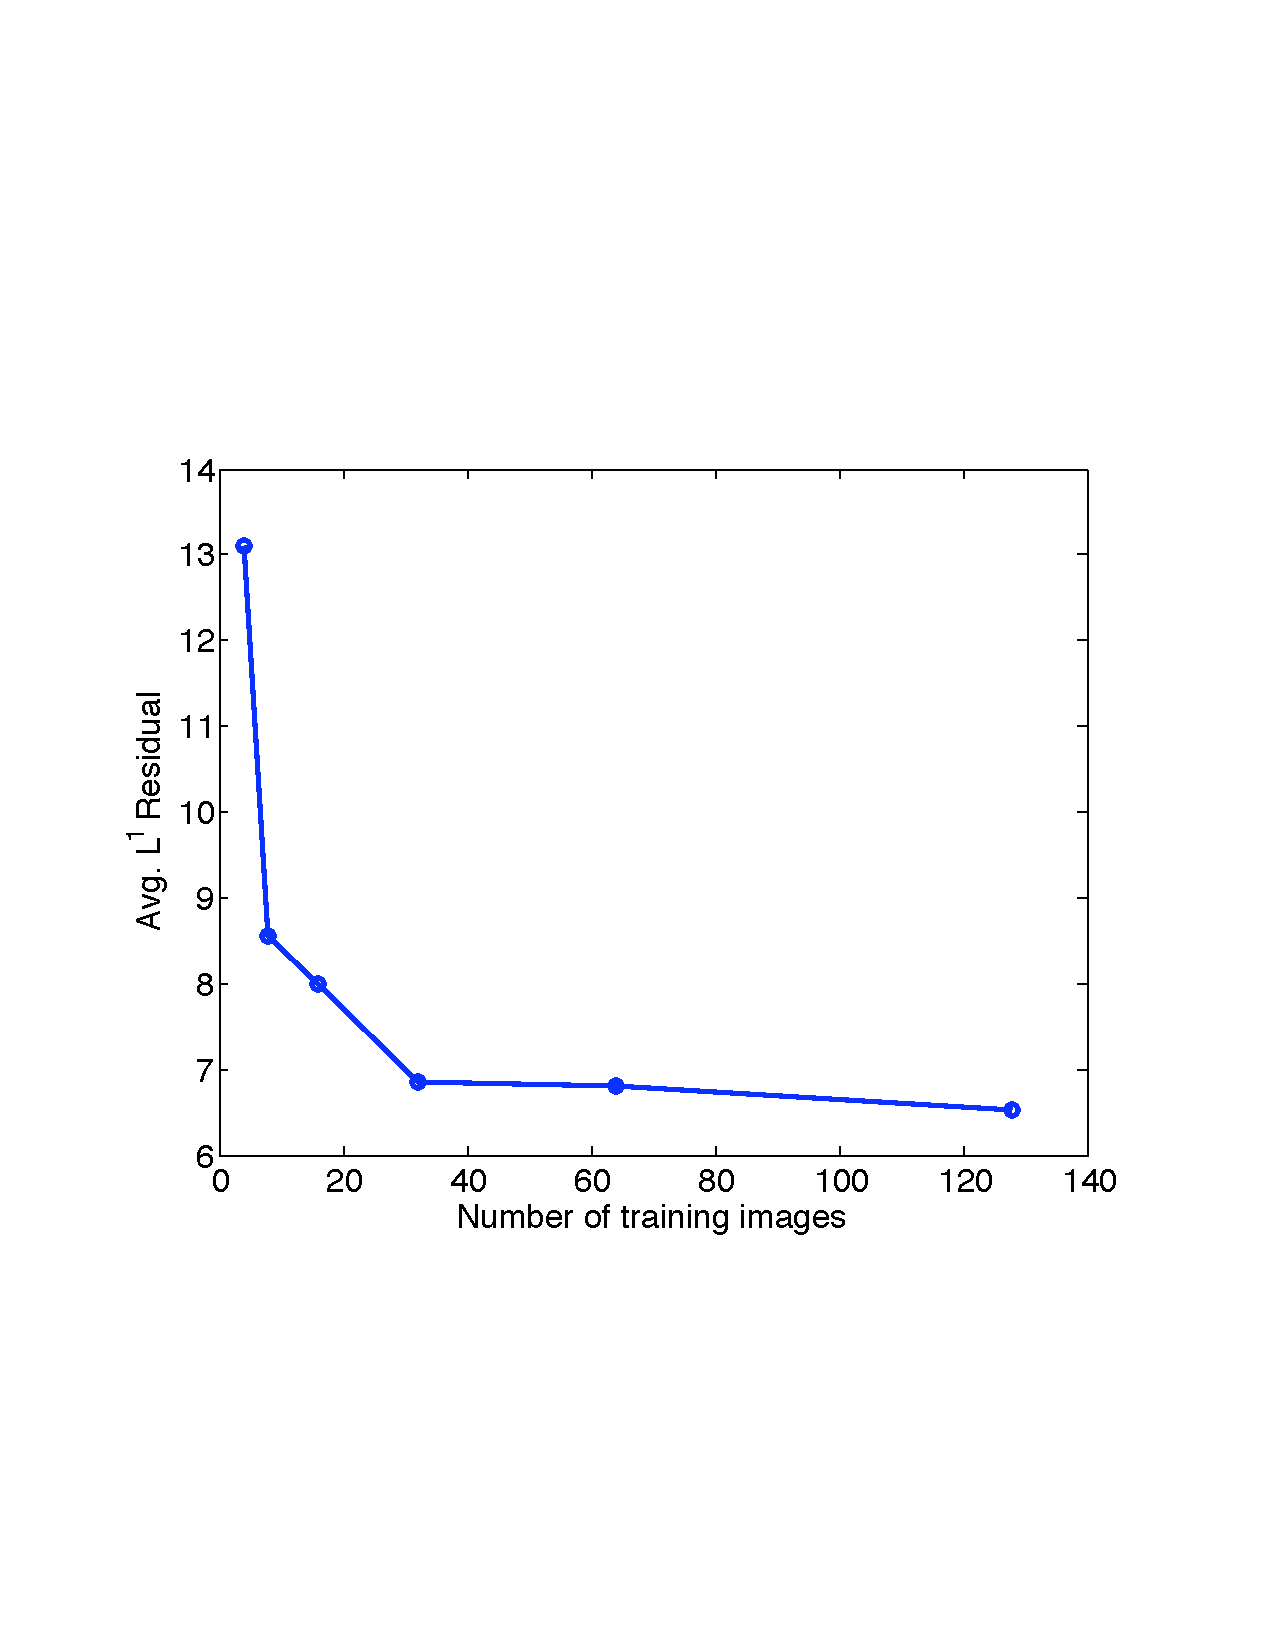
\includegraphics[\imagesizestring=\imagesizea]{figures_cvpr/illum_results/granularity_sunset.pdf} &
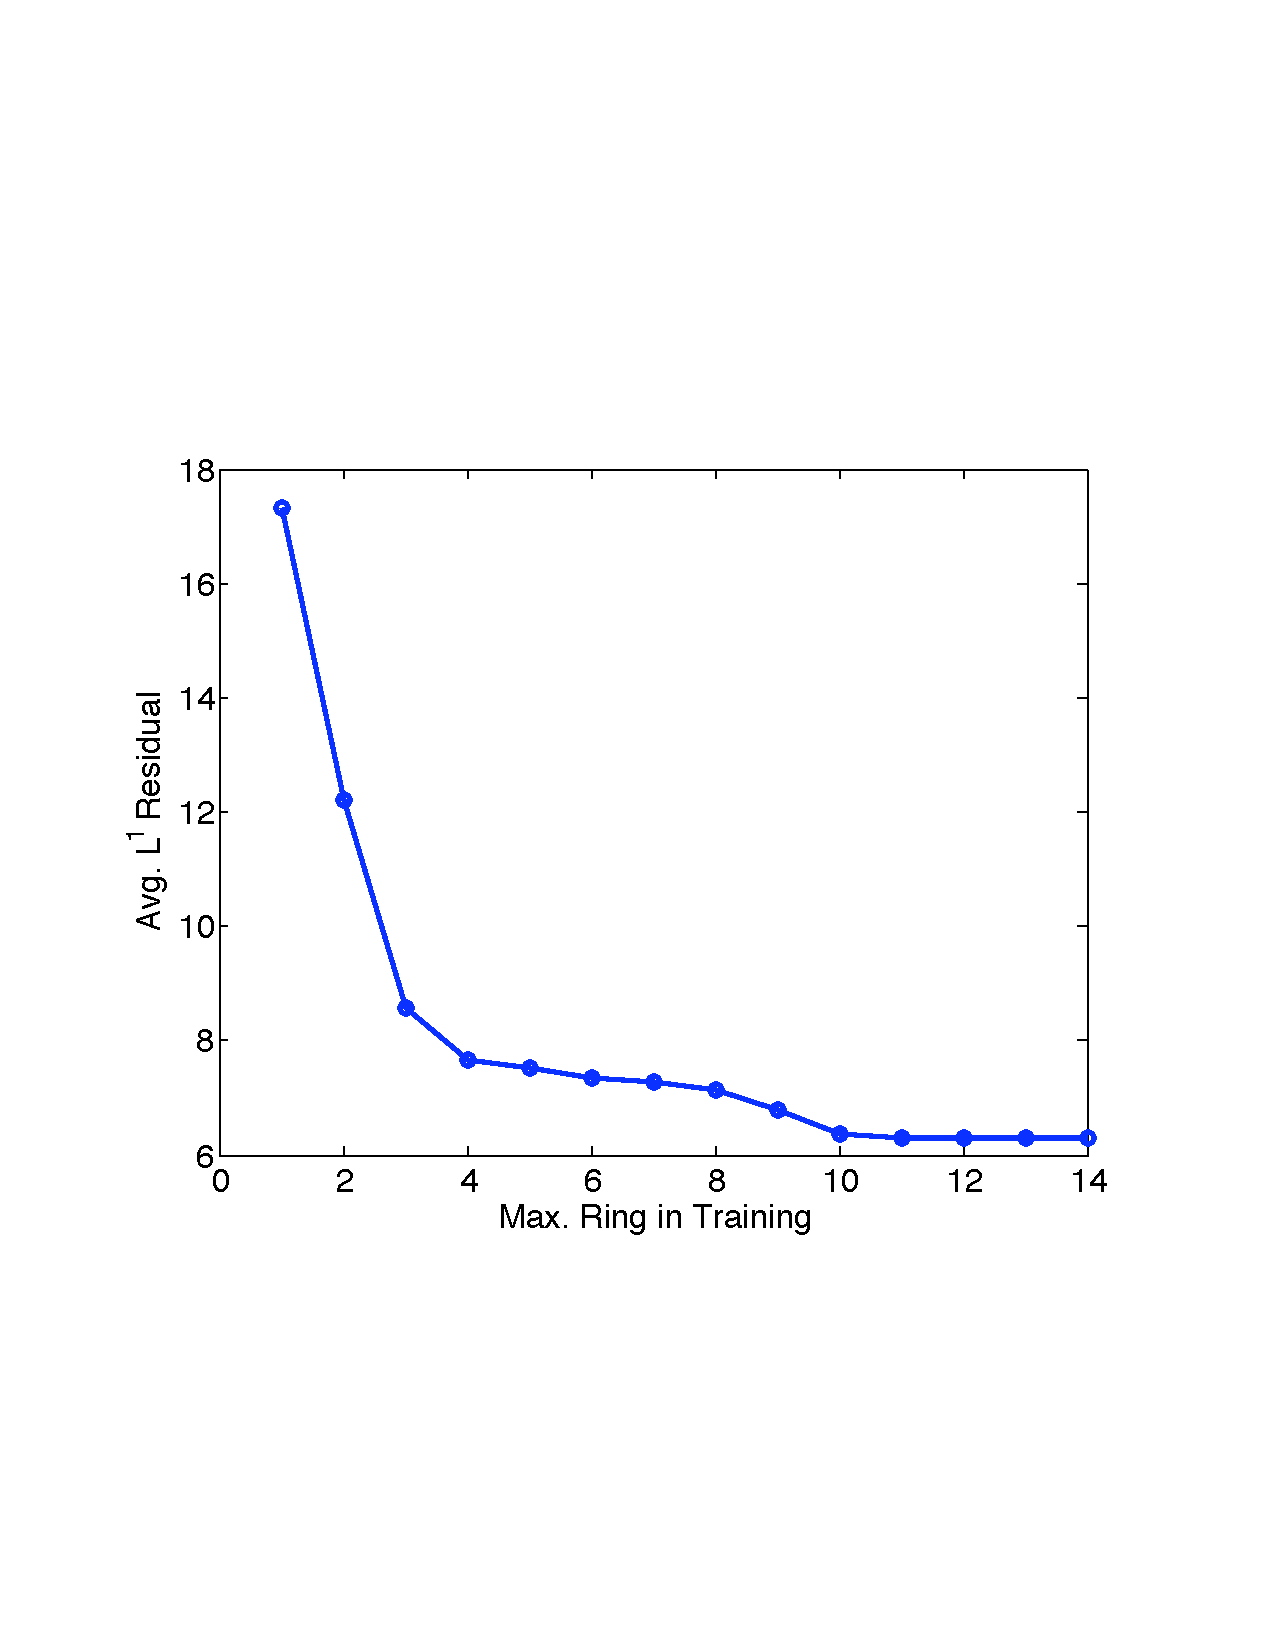
\includegraphics[\imagesizestring=\imagesizea]{figures_cvpr/illum_results/coverage_sunset.pdf} \\
(a) Granularity & (b) Coverage
\end{tabular}\vspace{2mm}
\end{center}
}

\frame{
\renewcommand{\imagesizestring}{height}
\renewcommand{\imagesizea}{0.41\textheight}
\frametitle{Final Illuminations}
\begin{tabular}{cc}
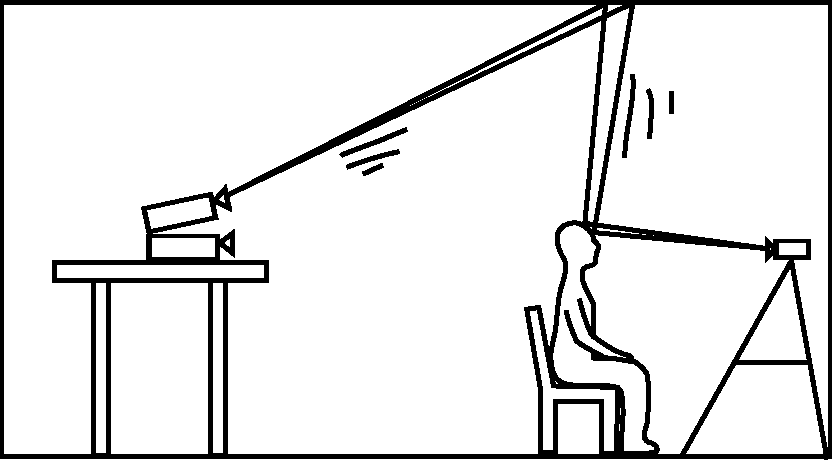
\includegraphics[\imagesizestring = \imagesizea]{images/camera_rig_drawings/side_front.pdf} & 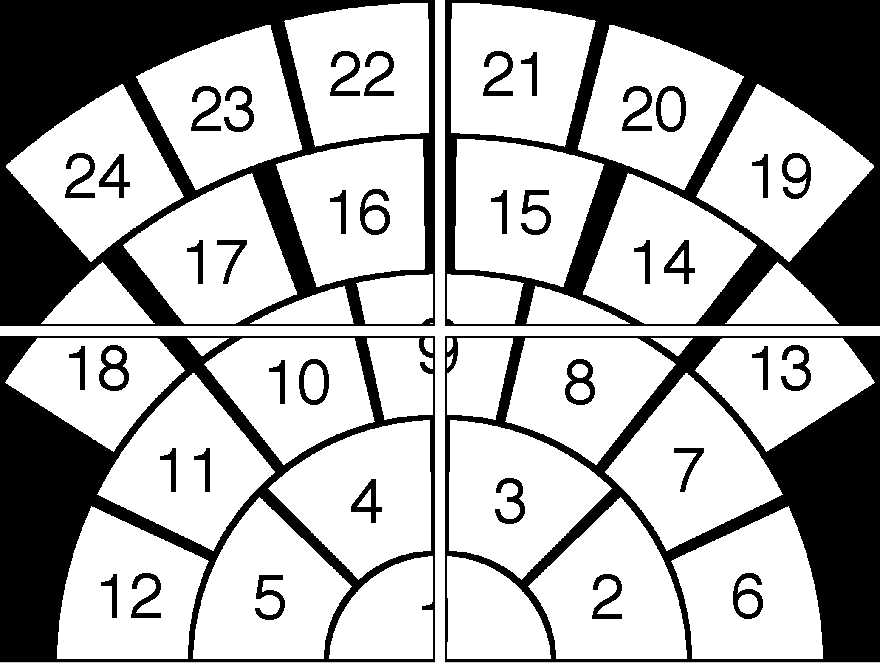
\includegraphics[\imagesizestring = \imagesizea]{images/illuminations/front.png}\\
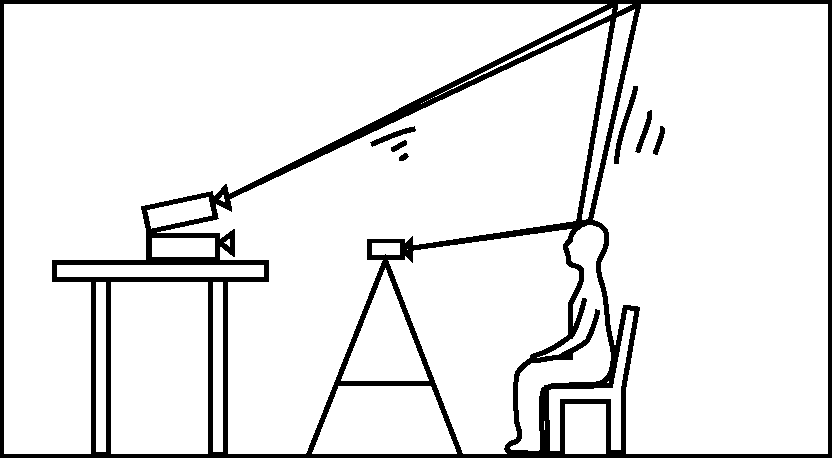
\includegraphics[\imagesizestring = \imagesizea]{images/camera_rig_drawings/side_back.pdf} & 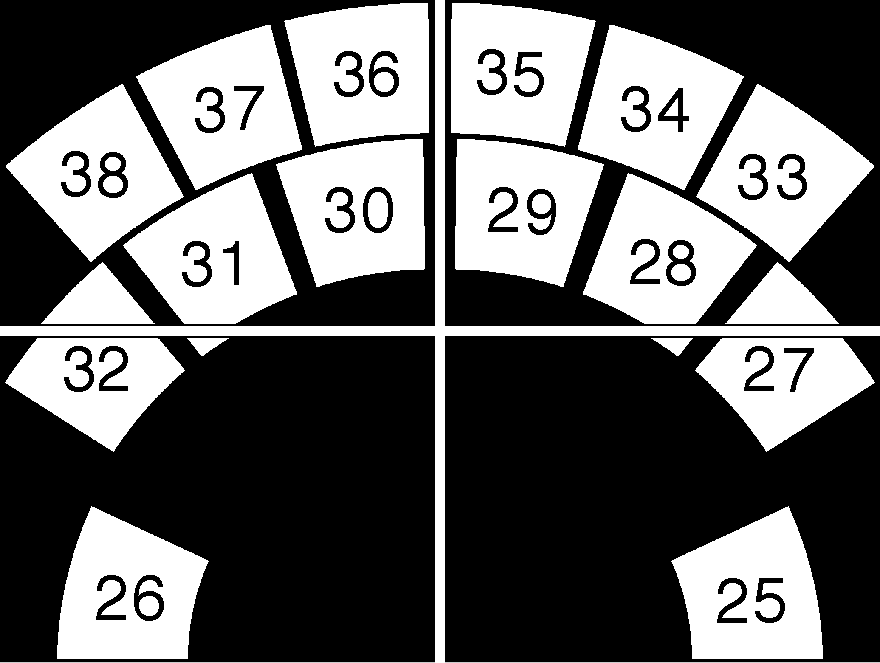
\includegraphics[\imagesizestring = \imagesizea]{images/illuminations/back.png}
\end{tabular}
}


\frame{\frametitle{Sample Training Images, Originals}
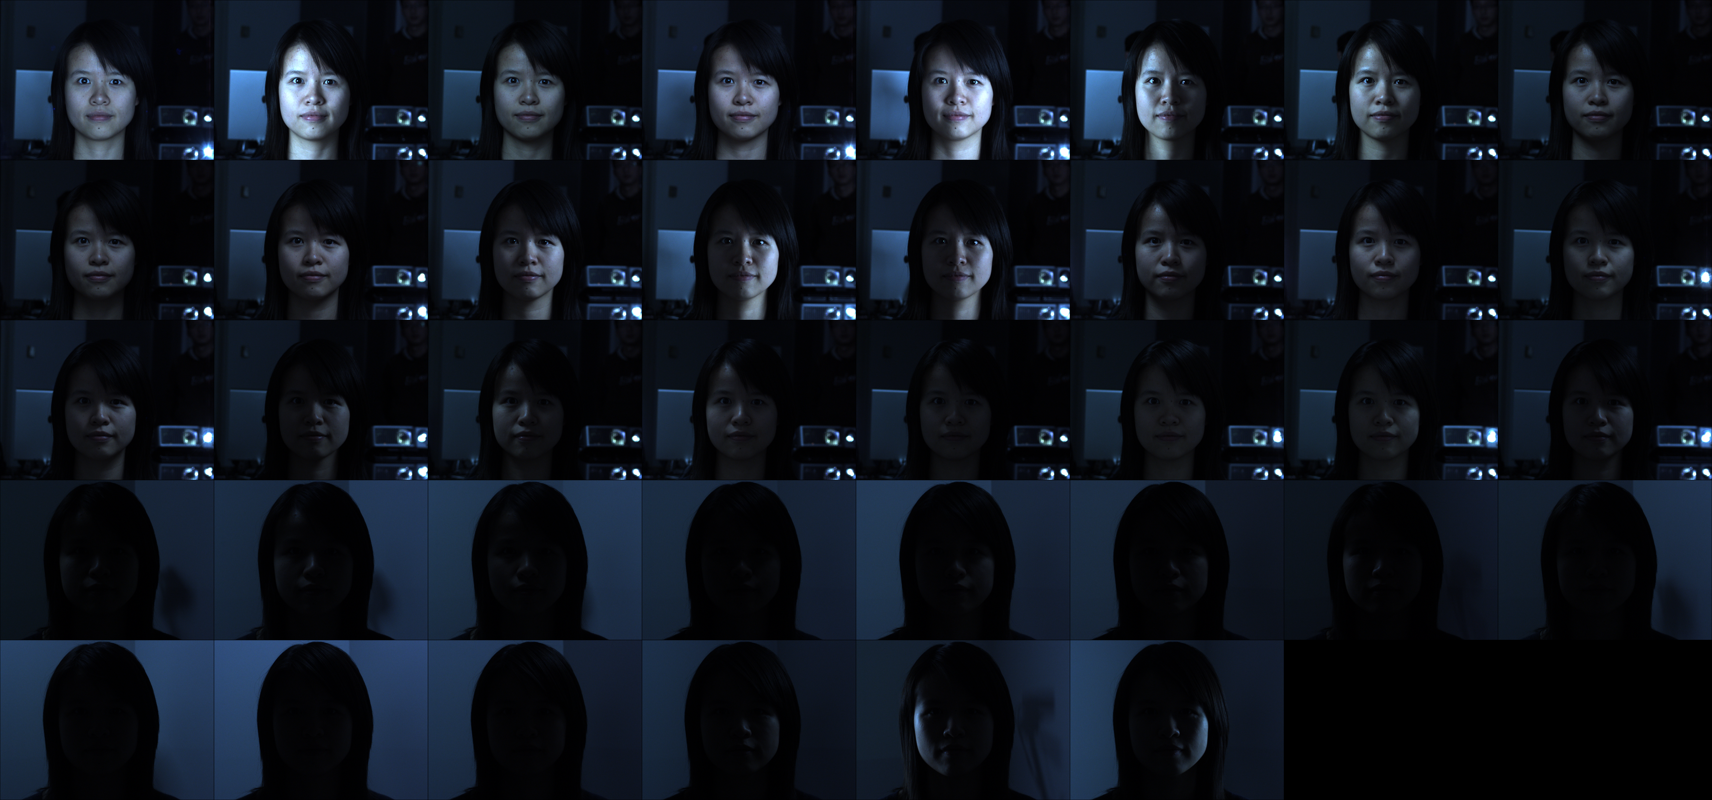
\includegraphics[width=\textwidth]{images/training_contact_sheet.png}
}

%\frame{\frametitle{Sample Training Images, Aligned and Cropped}
%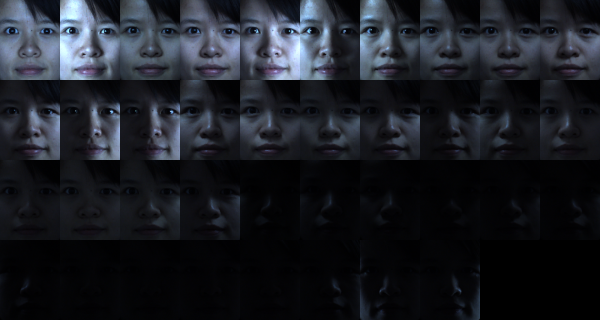
\includegraphics[width=\textwidth]{images/training_contact_sheet_cropped.png}
%}



\section{Alignment}
\frame{\tableofcontents[currentsection, currentsubsection]}
%!TEX root = prelim.tex
%!TEX root = fakeroot.tex


% Alignment
\subsection{Sparse Representation with Warping}
\frame{\frametitle{Compound Effect of Alignment and Illumination}
\renewcommand{\imagesizestring}{height}
\renewcommand{\imagesizea}{0.25\textheight}
\renewcommand{\imagesizeb}{0.15\textheight}
\renewcommand{\gapsizea}{-0mm}
\begin{tabular}[b]{cc@{}b{.5\textwidth}}
% Example for setting the heights of the images
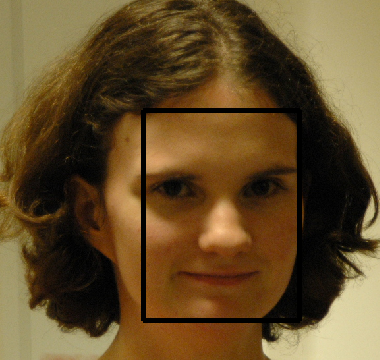
\includegraphics[\imagesizestring=\imagesizea]{figures_cvpr/promo/case1/detector.png}& \hspace{\gapsizea}
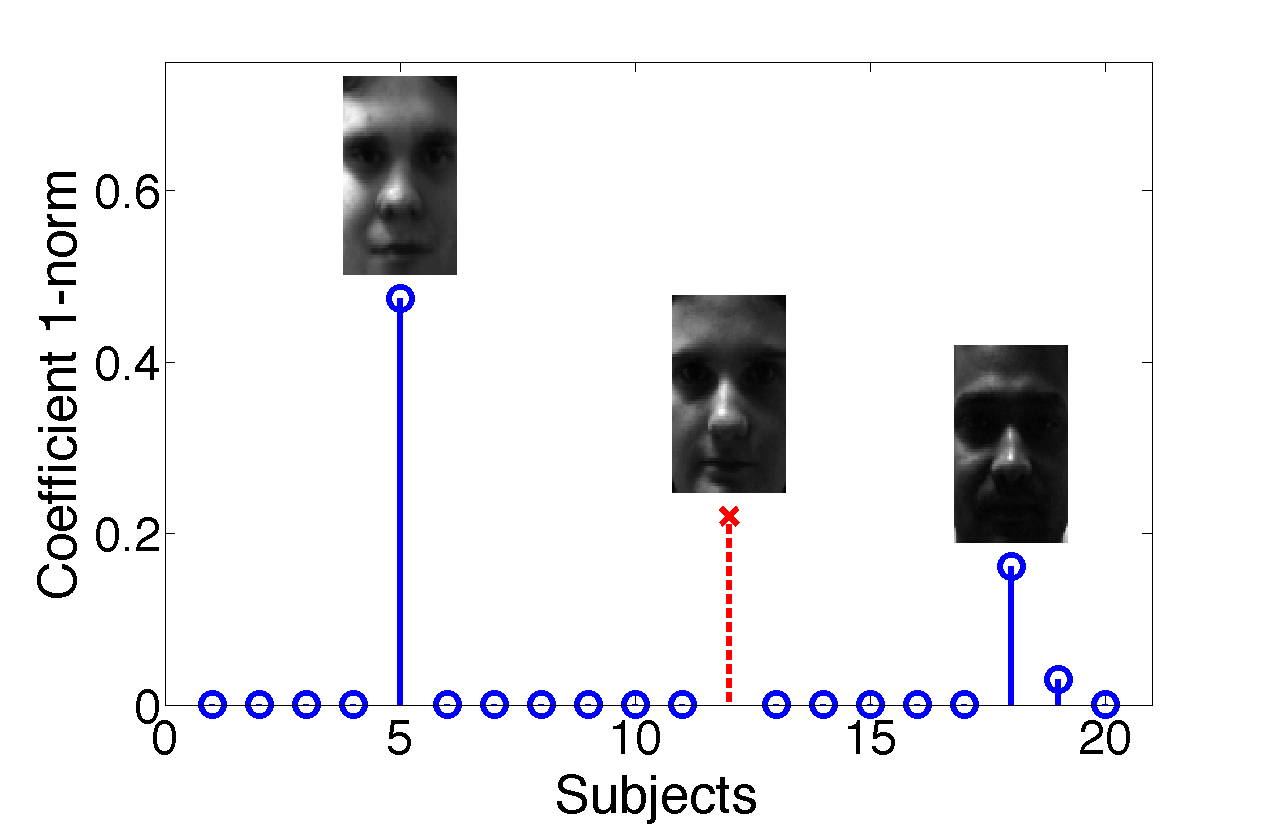
\includegraphics[\imagesizestring=\imagesizea]{figures_cvpr/promo/case1/sci_with_axis_face_case1.png} & 
{\bf Poor alignment}, Sufficient training illuminations \vfill\\
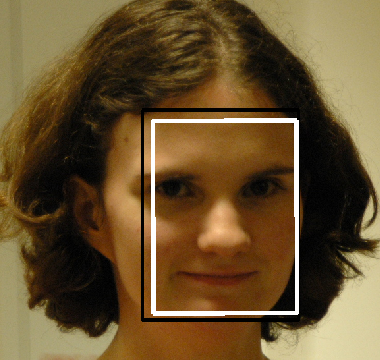
\includegraphics[\imagesizestring=\imagesizea]{figures_cvpr/promo/alignment_and_detector.png}& \hspace{\gapsizea}
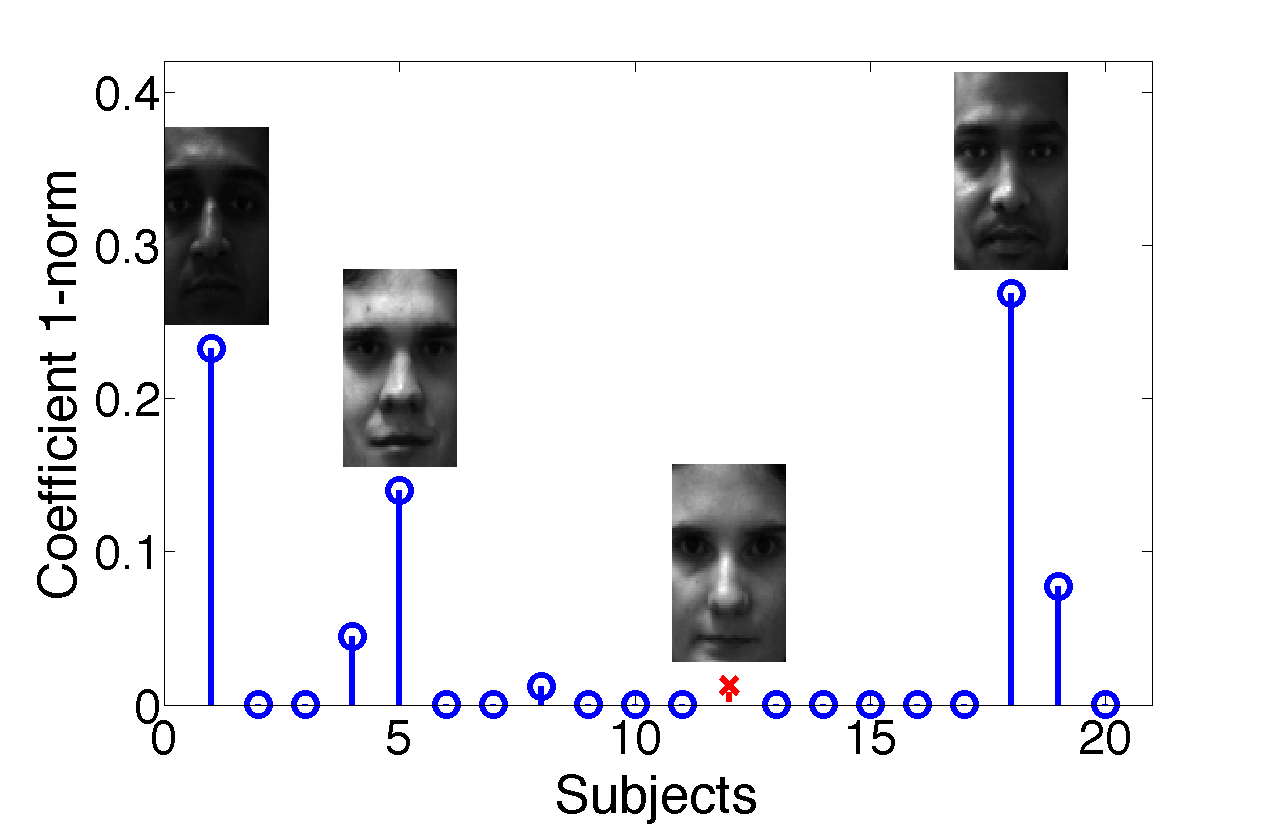
\includegraphics[\imagesizestring=\imagesizea]{figures_cvpr/promo/case2/sci_with_axis_face_case2.png} & 
{{\bf Good alignment}, Insufficient training illuminations}\vfill\\
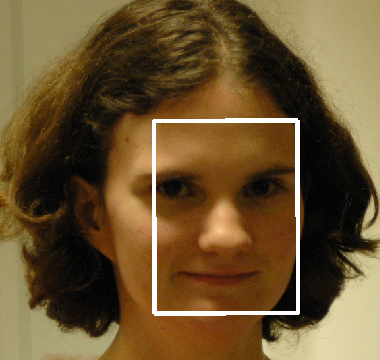
\includegraphics[\imagesizestring=\imagesizea]{figures_cvpr/promo/case3/alignment.png} & \hspace{\gapsizea}
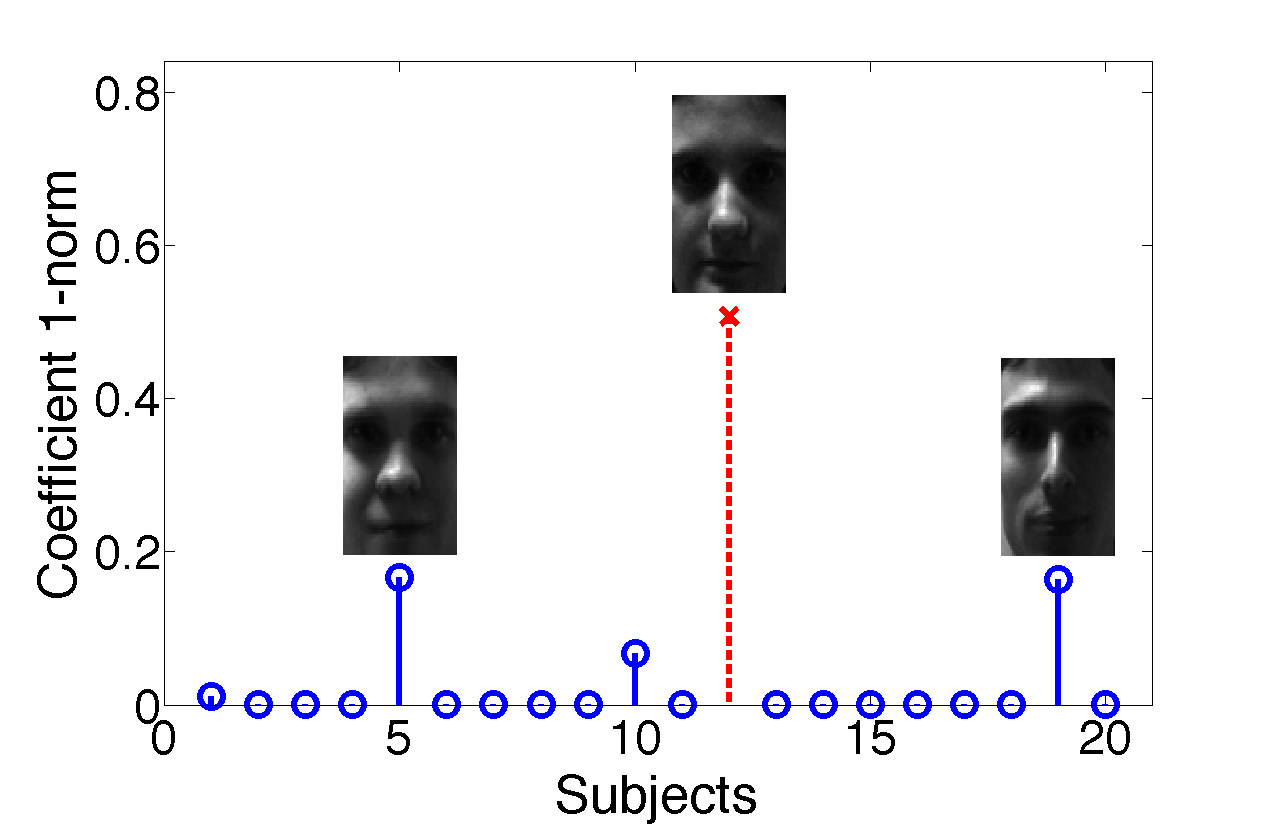
\includegraphics[\imagesizestring=\imagesizea]{figures_cvpr/promo/case3/sci_with_axis_face_case3.png} &
{{\bf Good alignment}, Sufficient training illuminations}\vfill
\end{tabular}
}

\frame{
\frametitle{Image Embedding}
\vspace{-3mm}
\begin{center}
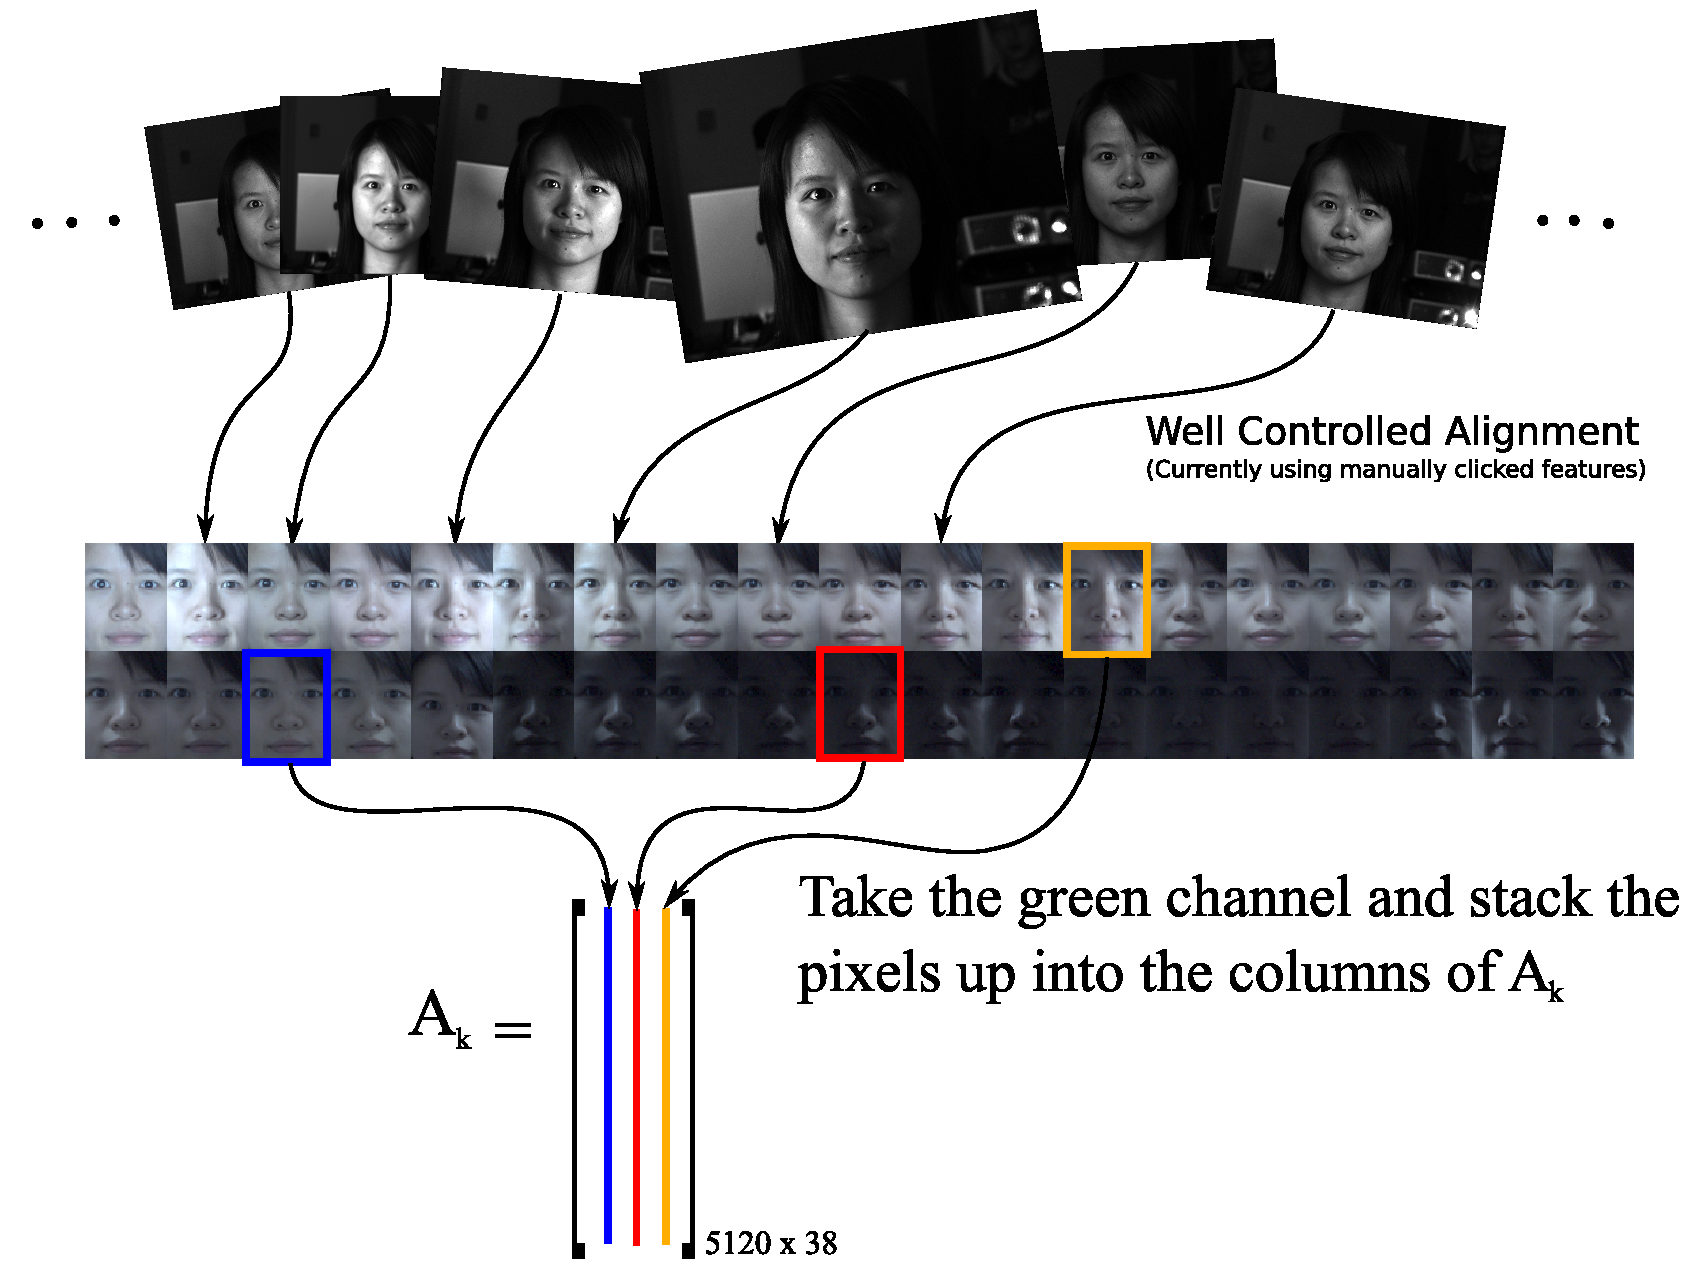
\includegraphics[width=.70\textwidth]{figures_embedding/training_embedding.pdf}\\
$A = [ A_1 \mid A_2 \mid \dots \mid A_K ] \in \Re^{m \times n}$
\end{center}
}

\frame{
\frametitle{Sparse Representation with Warping}
\vspace{-.1in} {\footnotesize
\begin{itemize}
\item<1-> SRC uses the following minimization:
\begin{equation*}
(\hat{\x}, \hat{\e}) = \argmin{\x,\e} \| \x \|_1 + \| \e\|_1 \quad \subj \quad \underbrace{\y_0}_{\mbox{\tiny test image}} = \underbrace{A}_{\mbox{\tiny training data}} \underbrace{\x}_{\mbox{\tiny coefficients}} + \underbrace{\e}_{\mbox{\tiny sparse error}}
\end{equation*}
\begin{center}{\color{blue} Assumes $\y$ aligned}\end{center}
\item<2-> For an un-aligned test image:
\begin{equation*}
(\hat{\x}, \hat{\e}, \hat{\tau}) = \argmin{\x,\e,\tau \in T} \| \x \|_1 + \| \e \|_1 \quad \subj \quad  \underbrace{\y}_{\mbox{\tiny un-aligned}} \circ \underbrace{\tau}_{\mbox{\tiny transformation}} = A \x + \e
\end{equation*}
\begin{center}{\color{blue}many local minima! scales badly!}\vspace{-.05in}\end{center}
\item<3-> Per-User alignment:
\begin{equation*}
(\hat \x, \hat \e,\hat \tau_i) = \argmin{\x,\e,\tau_i \in T} \| \e \|_1 \quad \subj \quad \y \circ \tau_i = A_i \x + \e
\end{equation*}
\begin{center}{\color{blue}not convex!}\vspace{-.05in}\end{center}
\item<4-> Linearize w.r.t. parameterization of $\tau$:
\begin{equation*}
(\hat \x, \hat \e, \Delta\hat\tau_i) = \argmin{\x,\e,\Delta\tau_i \in T} \| \e \|_1 \quad \subj \quad \y\circ \tau + \underbrace{J}_{\mbox{\tiny Jacobian}} \Delta \tau_i = A_i \x + \e
\end{equation*}
\end{itemize}
}}

\frame{
\frametitle{Iterative Alignment}
\begin{itemize}
\item Since we linearized $\y \circ \tau_i$, we have to iterate between solving
\begin{eqnarray*}
(\hat \x, \hat \e, \Delta\hat\tau_i) &\leftarrow& \argmin{\x,\e,\Delta\tau_i \in T} \| \e \|_1 \quad \subj \quad \y\circ \tau_i + J \Delta \tau_i = A_i \x + \e \\
\tau_i &\leftarrow& \tau_i + \Delta\hat \tau_i
\end{eqnarray*}
and re-computing the Jacobian $J$ about the new point $\y\circ (\tau_i + \Delta \tau_i)$.
\item To avoid degenerate solutions, normalize the {\em warped} test image:
\begin{equation*}
\tilde\y(\tau) = \frac{\y\circ\tau}{||\y\circ\tau||_2}
\end{equation*}
\item Normalize columns of $A$ to unit $\ell^2$ norm.
\item Enforce constraint $\x>0$.
\item Can extend this to multiscale
\end{itemize}
}

\frame{
\frametitle{Recognition Step}
\begin{itemize}
\item Re-sample training database using inverted $\tau_i$ from alignment step:
\begin{equation*}
A \leftarrow \left[ A_1 \circ \tau_1^-1 \ldots A_i \circ \tau_i^-1\ldots \right]
\end{equation*}
\item Perform global optimization:
\begin{equation*}
(\hat{\x}, \hat{\e}) = \argmin{\x,\e} \| \x \|_1 + \| \e\|_1 \quad \subj \quad \y = \underbrace{A}_{\mbox{\tiny aligned}} \x + \e
\end{equation*}
\item Return user with lowest residual $||\y - A_i \hat x_i||_2$. 
\end{itemize}
}

\frame{
\frametitle{Recognition Pipeline}
\begin{center}
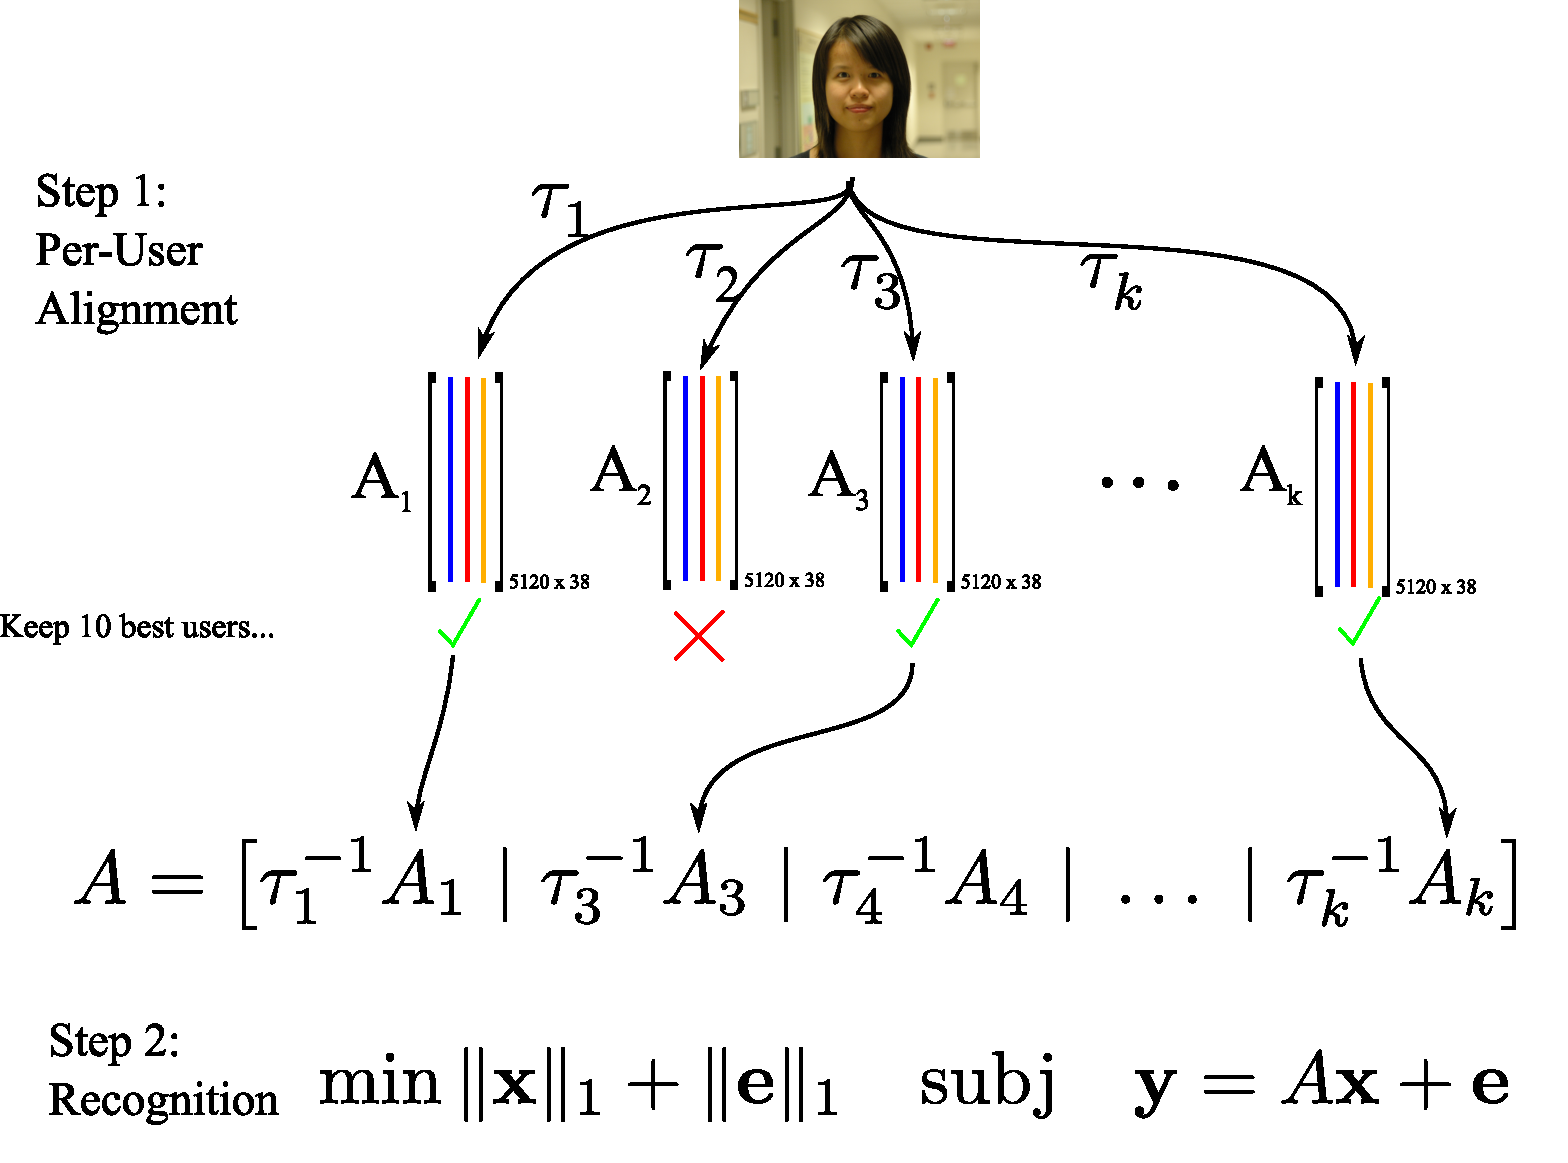
\includegraphics[width=.75\textwidth]{figures_embedding/pipeline.pdf}
\end{center}
}


%\frame{\frametitle{Alignment Examples}
%$\ell^1$ and $\ell^2$ minimization alignment comparison
%\begin{columns}
%\begin{column}{0.5\textwidth}
%\renewcommand{\imagesizestring}{height}
%\renewcommand{\imagesizea}{0.2\textheight}
%\begin{tabular}[t]{@{}c@{}c@{}c@{}c@{}m{.2\textwidth}}
%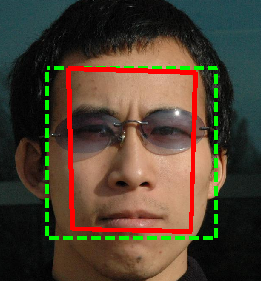
\includegraphics[\imagesizestring=\imagesizea]{figures_cvpr/L1_cropped} &
%
\includegraphics[\imagesizestring=\imagesizea]{figures_cvpr/y_warp_L1} &
%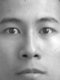
\includegraphics[\imagesizestring=\imagesizea]{figures_cvpr/y_hat_L1} &
%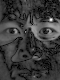
\includegraphics[\imagesizestring=\imagesizea]{figures_cvpr/e_L1} &
%$\|\e\|_1$\\[-.05in]
%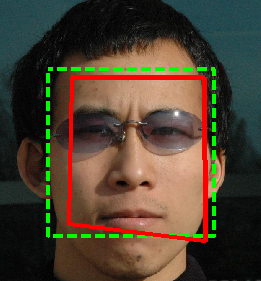
\includegraphics[\imagesizestring=\imagesizea]{figures_cvpr/L2_cropped} &
%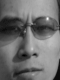
\includegraphics[\imagesizestring=\imagesizea]{figures_cvpr/y_warp_L2} &
%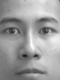
\includegraphics[\imagesizestring=\imagesizea]{figures_cvpr/y_hat_L2} &
%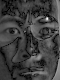
\includegraphics[\imagesizestring=\imagesizea]{figures_cvpr/e_L2} &
%$\|\e\|_2$ \\[-.1in]
%{\tiny Face Boundary} & {\tiny Aligned Test} & {\tiny Reconstruction} & {\tiny $|$Error$|$}
%\end{tabular}
%\end{column}
%\begin{column}{0.5\textwidth}
%\renewcommand{\imagesizestring}{height}
%\renewcommand{\imagesizea}{0.2\textheight}
%Alignment tolerance for out-of-plane pose variation
%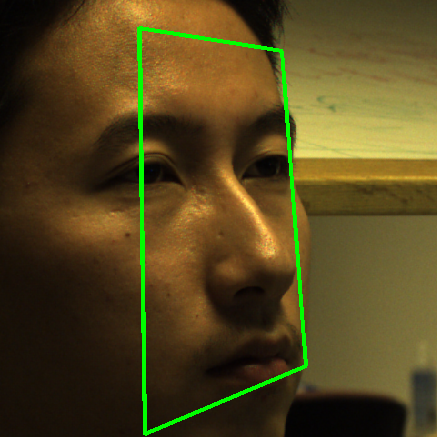
\includegraphics[\imagesizestring=\imagesizea]{figures_cvpr/21}
%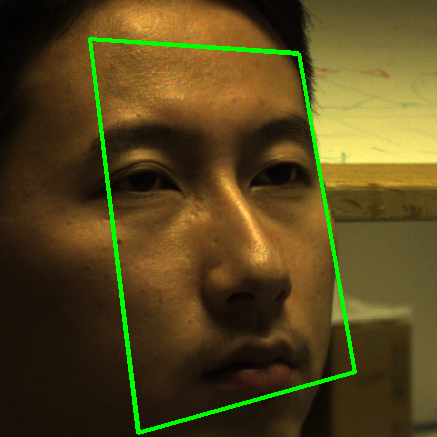
\includegraphics[\imagesizestring=\imagesizea]{figures_cvpr/19}
%
\includegraphics[\imagesizestring=\imagesizea]{figures_cvpr/17}
%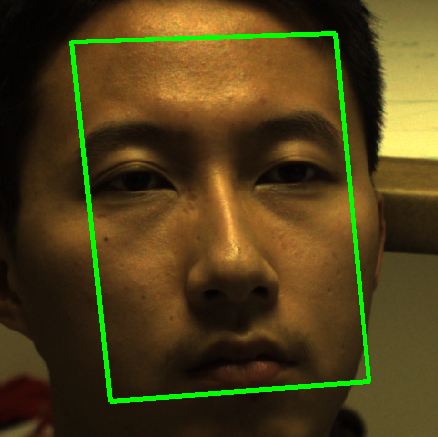
\includegraphics[\imagesizestring=\imagesizea]{figures_cvpr/15}
%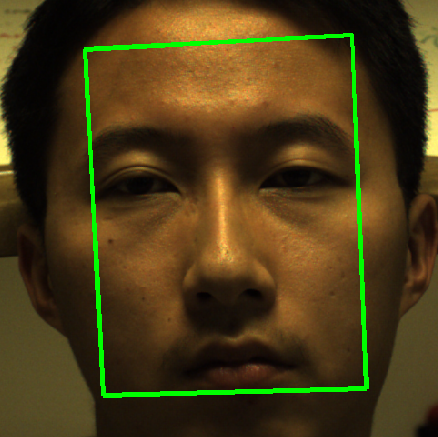
\includegraphics[\imagesizestring=\imagesizea]{figures_cvpr/13}\\
%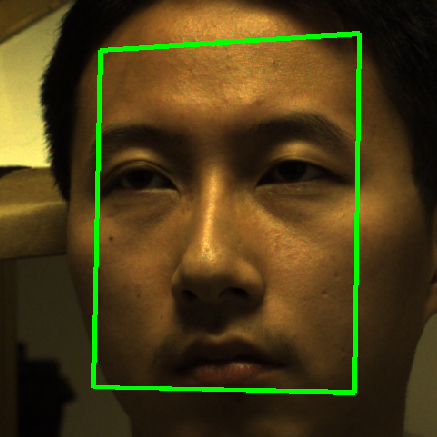
\includegraphics[\imagesizestring=\imagesizea]{figures_cvpr/11}
%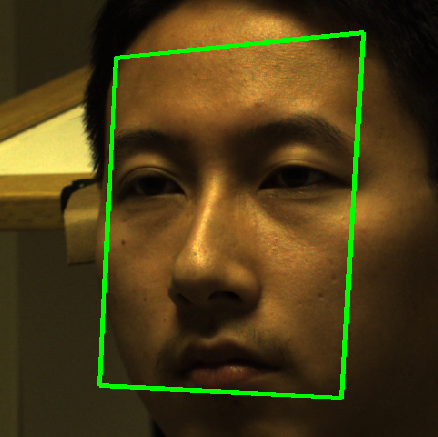
\includegraphics[\imagesizestring=\imagesizea]{figures_cvpr/09}
%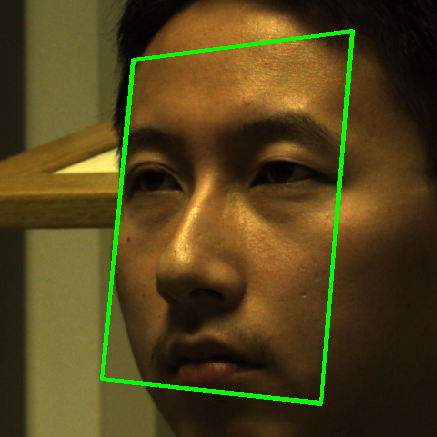
\includegraphics[\imagesizestring=\imagesizea]{figures_cvpr/7}
%\includegraphics[\imagesizestring=\imagesizea]{figures_cvpr/5}
%\includegraphics[\imagesizestring=\imagesizea]{figures_cvpr/3}\\
%Alignment using a projective transformation works up to about $45^{\circ}$.
%\end{column}
%\end{columns}
%}

\subsection{Experiments}




\renewcommand{\imagesizestring}{height}
\renewcommand{\imagesizea}{0.36\textheight}
\renewcommand{\gapsizea}{-0mm}
\frame{\frametitle{Alignment region of attraction}
%\begin{tabular}{cc}
\begin{center}
\includegraphics[\imagesizestring=\imagesizea]{figures_cvpr/promo/alignment_and_detector.png}
\includegraphics[\imagesizestring= \imagesizea]{figures_cvpr/translation_fig3.png}
\includegraphics[\imagesizestring= \imagesizea]{figures_cvpr/translation_rotation_fig1.png}
\end{center}
%\end{tabular}
\vspace{0mm}
{\tiny
\begin{itemize}
\item Translation is expressed as a fraction of outer eye corner distance.
\item In-plane rotation is expressed in degrees. 
\item Probability of convergence from synthetic transformations to hand-clicked ground truth
\item Training: CMU Multi-PIE, 120 subjects, 11 illuminations, session 2.  Re-sampled to $60 \times 80$ pixels.
\item Testing: 1 new illumination from session 3
\item Viola Jones' face detector average error on this data set falls safely within our region of attraction
\end{itemize}}
}


\frame{\frametitle{Alignment Examples}
{\footnotesize
\vspace{-.1in}
Comparison of $\ell^1$ and $\ell^2$ minimization:
\renewcommand{\imagesizestring}{height}
\renewcommand{\imagesizea}{0.15\textheight}
\vspace{-.05in}
\begin{center}
\begin{tabular}[t]{b{.3in}cccc}
$\min \|\e\|_2$\vfill &
\includegraphics[\imagesizestring=\imagesizea]{figures_cvpr/L2_cropped} &
\includegraphics[\imagesizestring=\imagesizea]{figures_cvpr/y_warp_L2} &
\includegraphics[\imagesizestring=\imagesizea]{figures_cvpr/y_hat_L2} &
\includegraphics[\imagesizestring=\imagesizea]{figures_cvpr/e_L2} \\
$\min \|\e\|_1$\vfill &
\includegraphics[\imagesizestring=\imagesizea]{figures_cvpr/L1_cropped} &
\includegraphics[\imagesizestring=\imagesizea]{figures_cvpr/y_warp_L1} &
\includegraphics[\imagesizestring=\imagesizea]{figures_cvpr/y_hat_L1} &
\includegraphics[\imagesizestring=\imagesizea]{figures_cvpr/e_L1} \\
& {\tiny Face Boundary} & {\tiny Aligned Test} & {\tiny Reconstruction} & {\tiny $|$Error$|$}
\end{tabular}
\end{center}

%$\ell^1$ and $\ell^2$ minimization alignment comparison
\renewcommand{\imagesizestring}{height}
\renewcommand{\imagesizea}{0.15\textheight}
\vspace{-.1in}

%Alignment tolerance for out-of-plane pose variation
Alignment using a projective transformation works up to about $45^{\circ}$.
\vspace{-.05in}
\begin{center}
\includegraphics[\imagesizestring=\imagesizea]{figures_cvpr/21}
\includegraphics[\imagesizestring=\imagesizea]{figures_cvpr/19}
\includegraphics[\imagesizestring=\imagesizea]{figures_cvpr/17}
\includegraphics[\imagesizestring=\imagesizea]{figures_cvpr/15}
\includegraphics[\imagesizestring=\imagesizea]{figures_cvpr/13}\\
\includegraphics[\imagesizestring=\imagesizea]{figures_cvpr/11}
\includegraphics[\imagesizestring=\imagesizea]{figures_cvpr/09}
\includegraphics[\imagesizestring=\imagesizea]{figures_cvpr/7}
\includegraphics[\imagesizestring=\imagesizea]{figures_cvpr/5}
\includegraphics[\imagesizestring=\imagesizea]{figures_cvpr/3}\\
\end{center}}
}

%!TEX root = prelim.tex
%!TEX root = fakeroot.tex


\frame{\frametitle{Large Scale Multi PIE experiments}
\begin{center}
\begin{tabular}{|l|c|c|c|c|}
\hline
Rec. Rates & Session 2 & Session 3 & Session 4  \\
\hline
\hline
LDA$_d$ (LDA$_m$) & 5.1 (49.4)\%  & 5.9 (44.3)\% & 4.3 (47.9)\%  \\
\hline
NN$_d$ (NN$_m$)  & 26.4 (67.3)\% & 24.7 (66.2)\% & 21.9 (62.8)\%  \\
\hline
NS$_d$ (NS$_m$) &  30.8 (77.6)\% & 29.4 (74.3)\% & 24.6 (73.4)\% \\
\hline
{Algorithm 1} & {\bf 91.4} \% & {\bf 90.3} \% & {\bf 90.2} \% \\
\hline
\end{tabular}
\end{center}
\begin{columns}
\begin{column}{0.5\textwidth}
\begin{itemize}
{\footnotesize
\item Training: all 249 subj. from session 1\\7 frontal illuminations
\item Testing: all users, from sessions 2-4\\ all 20 illuminations 
\item Use the 88 users not in session 1 for validation
\item Our Algorithm 1 used face detector; no manual intervention
\item subscript m for manual alignment, subscript d for detector
\item neutral expression
}
\end{itemize}
\end{column}
\begin{column}{0.5\textwidth}
\begin{center}
\includegraphics[width=\textwidth]{figures_cvpr/roc3.png}
\end{center}
\end{column}
\end{columns}
}



%%%Cause of errors Our algorithm's errors are mostly caused by a few subjects who significantly change their appearances between sessions (such as hair, facial hair, and eyeglasses). Some representative examples are shown in %Figure \ref{fig:failed-examples}. In fact, for those subjects, alignment and recognition fail on almost all test illuminations.\vspace{0mm} %This may be due the limited number of illuminations present in the training. \vspace{0mm}
%%%\begin{figure}

\renewcommand{\imagesizestring}{width}
\renewcommand{\imagesizea}{0.16\textwidth}
\frame{
\frametitle{Representative examples of failed Multi-PIE subjects}
\includegraphics[\imagesizestring =\imagesizea]{figures_cvpr/079_01_01_051_08.png} 
\includegraphics[\imagesizestring =\imagesizea]{figures_cvpr/130_01_01_051_08.png}
\includegraphics[\imagesizestring =\imagesizea]{figures_cvpr/163_01_01_051_08.png} 
\includegraphics[\imagesizestring =\imagesizea]{figures_cvpr/175_01_01_051_08.png} 
\includegraphics[\imagesizestring =\imagesizea]{figures_cvpr/118_01_01_051_08.png} 
\includegraphics[\imagesizestring =\imagesizea]{figures_cvpr/223_01_01_051_08.png}\\
\includegraphics[\imagesizestring =\imagesizea]{figures_cvpr/079_02_01_051_08.png} 
\includegraphics[\imagesizestring =\imagesizea]{figures_cvpr/130_02_01_051_08.png} 
\includegraphics[\imagesizestring =\imagesizea]{figures_cvpr/163_02_01_051_08.png} 
\includegraphics[\imagesizestring =\imagesizea]{figures_cvpr/175_02_01_051_08.png} 
\includegraphics[\imagesizestring =\imagesizea]{figures_cvpr/118_02_01_140_08.png} 
\includegraphics[\imagesizestring =\imagesizea]{figures_cvpr/223_02_01_140_08.png}\\
Trouble when large changes in the appearance between training and testing
\begin{itemize}
\item Hair color, hair style
\item Eyeglasses
\item Facial Hair
\end{itemize}
}

% Experiments on our own training images

\renewcommand{\imagesizestring}{width}
\renewcommand{\imagesizea}{0.2\textwidth}
\frame{\frametitle{Experiments on our data set}
\small{
Training (common to all): 74 users, 38 images per user
\includegraphics[\imagesizestring =\imagesizea]{figures_cvpr/examples/1/DSC_1319.JPG} 
\includegraphics[\imagesizestring =\imagesizea]{figures_cvpr/examples/1/DSC_1531.JPG} 
\includegraphics[\imagesizestring =\imagesizea]{figures_cvpr/examples/1/DSC_1574.JPG} 
\includegraphics[\imagesizestring =\imagesizea]{figures_cvpr/examples/1/DSC_1622.JPG} 
\includegraphics[\imagesizestring =\imagesizea]{figures_cvpr/examples/1/DSC_1786.JPG}\\
Testing: 242 images of 47 subjects, no glasses, frontal view $\Rightarrow \textbf{\color{red} 95.9\%}$ recognition.
\includegraphics[\imagesizestring =\imagesizea]{figures_cvpr/examples/2/DSC_1448.JPG} 
\includegraphics[\imagesizestring =\imagesizea]{figures_cvpr/examples/2/DSC_1585.JPG} 
\includegraphics[\imagesizestring =\imagesizea]{figures_cvpr/examples/2/DSC_1588.JPG} 
\includegraphics[\imagesizestring =\imagesizea]{figures_cvpr/examples/2/DSC_1666.JPG} 
\includegraphics[\imagesizestring =\imagesizea]{figures_cvpr/examples/2/DSC_1874.JPG}\\
Testing: 109 images of 23 subjects with eyeglasses  $\Rightarrow \textbf{\color{red} 91.5\%}$ recognition.
\includegraphics[\imagesizestring =\imagesizea]{figures_cvpr/examples/3/DSC_1572.JPG} 
\includegraphics[\imagesizestring =\imagesizea]{figures_cvpr/examples/3/DSC_1587.JPG} 
\includegraphics[\imagesizestring =\imagesizea]{figures_cvpr/examples/3/DSC_1623.JPG} 
\includegraphics[\imagesizestring =\imagesizea]{figures_cvpr/examples/3/DSC_1652.JPG} 
\includegraphics[\imagesizestring =\imagesizea]{figures_cvpr/examples/3/DSC_1675.JPG}\\
Testing: 19 images of 14 subjects with sunglasses $\Rightarrow \textbf{\color{red}63.2\%}$ recognition.
}}





\section{Occlusion}
\frame{\tableofcontents[currentsection, currentsubsection]}
%!TEX root = prelim.tex
%!TEX root = fakeroot.tex
\subsection{Contiguous Occlusion}

\renewcommand{\imagesizestring}{height}
\renewcommand{\imagesizea}{0.25\textheight}
\renewcommand{\imagesizeb}{0.15\textheight}


\frame{\frametitle{SRC on Random Corruption}
\renewcommand{\imagesizestring}{height}
\renewcommand{\imagesizea}{0.10\textheight}
\vspace{-.1in}
\begin{itemize}
\item<1-> SRC is provably optimal for {\em randomized} corruption. 
\begin{center}
\begin{columns}
\begin{column}{0.5\textwidth}
%{\footnotesize Yale Dataset, 19 images per person:}
\begin{center}
\begin{tabular}{@{}cccc@{}}
\includegraphics[\imagesizestring=\imagesizea]{IEEEPAMI_Occlusion/figures/ysp-30-125-o.pdf} &
\includegraphics[\imagesizestring=\imagesizea]{IEEEPAMI_Occlusion/figures/ysp-30-125-e.pdf} &
\includegraphics[\imagesizestring=\imagesizea]{IEEEPAMI_Occlusion/figures/ysp-30-125-w.pdf} &
\includegraphics[\imagesizestring=\imagesizea]{IEEEPAMI_Occlusion/figures/ysp-30-125-r.pdf} \\[-.05in]
\includegraphics[\imagesizestring=\imagesizea]{IEEEPAMI_Occlusion/figures/ysp-50-379-o.pdf} &
\includegraphics[\imagesizestring=\imagesizea]{IEEEPAMI_Occlusion/figures/ysp-50-379-e.pdf} &
\includegraphics[\imagesizestring=\imagesizea]{IEEEPAMI_Occlusion/figures/ysp-50-379-w.pdf} &
\includegraphics[\imagesizestring=\imagesizea]{IEEEPAMI_Occlusion/figures/ysp-50-379-r.pdf} \\[-.05in]
\includegraphics[\imagesizestring=\imagesizea]{IEEEPAMI_Occlusion/figures/ysp-70-80-o.pdf} &
\includegraphics[\imagesizestring=\imagesizea]{IEEEPAMI_Occlusion/figures/ysp-70-80-e.pdf} &
\includegraphics[\imagesizestring=\imagesizea]{IEEEPAMI_Occlusion/figures/ysp-70-80-w.pdf} &
\includegraphics[\imagesizestring=\imagesizea]{IEEEPAMI_Occlusion/figures/ysp-70-80-r.pdf}\\[-.1in]
{\tiny Test Image} & {\tiny Error} & {\tiny Coefficients} & {\tiny Reconstruction}
\end{tabular}
\end{center}
\end{column}
\begin{column}{0.5\textwidth}
\begin{center}
\includegraphics[height=.3\textheight]{IEEEPAMI_Occlusion/figures/yb_result_rc.pdf}\\
\end{center}
\end{column}
\end{columns}

\end{center}
%\vspace{.3in}
\item<2-> For contiguous occlusion, SRC can handle up to 30\% occlusion.\\
\begin{columns}
\begin{column}{0.5\textwidth}
\begin{center}
\begin{tabular}{@{}cccc@{}}
\includegraphics[\imagesizestring=\imagesizea]{IEEEPAMI_Occlusion/figures/352-30-o.pdf} &
\includegraphics[\imagesizestring=\imagesizea]{IEEEPAMI_Occlusion/figures/352-30-e.pdf}&
\includegraphics[\imagesizestring=\imagesizea]{IEEEPAMI_Occlusion/figures/352-30-w.pdf}&
\includegraphics[\imagesizestring=\imagesizea]{IEEEPAMI_Occlusion/figures/352-30-r.pdf} \\[-.05in]
\includegraphics[\imagesizestring=\imagesizea]{IEEEPAMI_Occlusion/figures/395-30-o.pdf} &
\includegraphics[\imagesizestring=\imagesizea]{IEEEPAMI_Occlusion/figures/395-30-e.pdf}&
\includegraphics[\imagesizestring=\imagesizea]{IEEEPAMI_Occlusion/figures/395-30-w.pdf} &
\includegraphics[\imagesizestring=\imagesizea]{IEEEPAMI_Occlusion/figures/395-30-r.pdf}\\[-.05in]
{\tiny Test Image} & {\tiny Error} & {\tiny Coefficients} & {\tiny Reconstruction}
\end{tabular}
\end{center}
\end{column}
\begin{column}{0.5\textwidth}
\begin{center}
\includegraphics[height=.3\textheight]{IEEEPAMI_Occlusion/figures/yb_result_bab.pdf}
\end{center}
\end{column}
\end{columns}
\item<2-> Can we do better for spatially contiguous occlusions?
\end{itemize}
}




%\includegraphics[width=2.9in]{IEEEPAMI_Occlusion/figures/yb_result_bab.pdf}




\frame{\frametitle{Markov Random Field Model}
\vspace{-.1in}
\begin{center}
\includegraphics[width=.35\textwidth]{images/lattice.pdf}\\
\vspace{-.15in}{\tiny Markov Random Field (MRF)}
\end{center}
\vspace{-.1in}
\begin{itemize}
\item Represent the image domain as an adjacency graph $G=(V,E)$
\item Let $\s\in \{-1,1\}^m$ be the support of $\e[i]$ :\\  $\s[i] = \left\{\begin{array}{cl} -1 & \mbox{for } \e[i] = 0\\ 1 & \mbox{for } \e[i] \neq 0 \end{array}\right.$
\item Model probability mass function of $\s$ using classical Ising model:
\begin{equation*}
p(\s) \propto \exp\Bigl\{\underbrace{\sum_{(i,j)\in E}\lambda_{ij}\s[i]\s[j]}_{\tiny \mbox{edge prior}} + \underbrace{\sum_{i\in V}\lambda_i \s[i]}_{\tiny \mbox{vertex prior}}\Bigr\}
\end{equation*}
\end{itemize}
}

\frame{\frametitle{Applying MRF to Occlusion}
\vspace{-.1in}
\begin{itemize}
\item Use simplified Ising Model: $p(\s) \propto \exp\Bigl\{\sum_{(i,j)\in E}\lambda \s[i]\s[j] \Bigr\}$
\item joint p.d.f of $\e$: \\ 
\vspace{-.15in}
\begin{eqnarray*}
p(\e,\s) &=& p(\s) p(\e|\s) = p(\s) \prod_i p(\e[i]|\s[i])\\  
&\propto&  \exp\Big\{\hspace{-0mm}\sum_{(i,j)\in E} \hspace{-0mm}\lambda\s[i]\s[j] + \sum_{i\in V} \log p(\e[i] \mid \s[i]) \Big\}
\end{eqnarray*}
\item approximate p($\e|\s$):\\
\begin{center}\includegraphics[width=0.5\textwidth]{figures_iccv/function.pdf}\end{center}
\end{itemize}
}

%\item Isolate effect of occlusion by assuming aligned images

%
%\frame{\frametitle{Solving Sparse Representation under MRF assumption}
%\begin{itemize}
%\item Want to solve 
%$\hat \s = \mbox{arg}\max_{\x_k,\e,\s} p(\s, \e) \quad \mbox{s.t.} \quad \y = A_k \x_k + \e.$
%\item Difficult non-convex optimization problem!
%\item $\Rightarrow$ alternate between: \begin{enumerate} 
%\item Performing sparse representation using pixels labeled as un-occluded: \\
%\begin{equation*}(\hat{\x}_k,\hat{\e}^*) = \argmin{\x,\e^*} \|\e^*\|_1  \; \textup{ s.t. } \; \y^* = A_k^*\x+\e^*, \x\geq 0 \end{equation*}
%\item Estimating the support of the occlusion given the representation error: \\
%\begin{equation*} \hat{\s} = \argmax{\s \in \{-1,1\}^m}  \sum_{(i,j)\in E}  \lambda \s[i]\s[j] + \sum_{i\in V} \log p(\e[i] | \s[i]).\end{equation*}
%\end{enumerate}
%\end{itemize}
%}

\frame{\frametitle{Solving Sparse Representation under MRF assumption}
\begin{itemize}
\item Want to solve 
$\hat \s = \mbox{arg}\max_{\x_k,\e,\s} p(\s, \e) \quad \mbox{s.t.} \quad \y = A_k \x_k + \e.$
\item Difficult non-convex optimization problem!
\item $\Rightarrow$ alternate between: \begin{enumerate} 
\item Solving $(\hat \x_k, \hat \e) = \mbox{arg}\max_{\x_k,\e} p(\s, \e) \quad \mbox{s.t.} \quad \y = A_k \x_k + \e.$\\
	 For very small $\tau$, this reduces (approximately) to solving SRC on a restricted domain:
	\begin{equation*}(\hat{\x}_k,\hat{\e}^*) = \argmin{\x,\e^*} \|\e^*\|_1  \; \textup{ s.t. } \; \y^* = A_k^*\x+\e^*, \x\geq 0 \end{equation*}
\item Solving $\hat \s = \mbox{arg}\max_{\s} p(\s, \e) \quad \mbox{s.t.} \quad \y = A_k \x_k + \e.$\\
	Under our assumptions this reduces to:
	\begin{equation*} \hat{\s} = \argmax{\s \in \{-1,1\}^m}  \sum_{(i,j)\in E}  \lambda \s[i]\s[j] + \sum_{i\in V} \log p(\e[i] | \s[i]).\end{equation*}
\end{enumerate}
\end{itemize}
}


\frame{\frametitle{The Complete MRF Recognition Algorithm}
{\footnotesize
\begin{algorithmic}[1]
\STATE {\bf Input:} A matrix of normalized training samples $A =
[A_1,A_2,\ldots,A_K] \in \Re^{m\times n}$ for $K$ classes, a test
sample $\y \in \Re^{m}$.

\FOR{each subject $k$}

\STATE Initialize the error support $\s^{(0)}_k = \mathbf{-1}_m$.

\STATE {\bf repeat}

\STATE \hspace{3mm}$A_k^* = A_k[\s^{(t-1)}_k=-1,\, :\, ]$, $\y^* =
\y[s^{(t-1)}_k=-1]$;

\STATE \hspace{3mm}Solve the convex program\\
\hspace{5mm} $(\hat{\x}_k,\hat{\e}^*) \;=\; \arg\min \|\e^*\|_1 $\\
\hspace{24mm} $\mathrm{ s.t. } \quad \y^* = A_k^*\x+\e^*, \, \x\geq 0;$

\STATE \hspace{3mm}$\hat{\e}_k\leftarrow \y-A_k\hat{\x}_k$;

\STATE \hspace{3mm}Update error support via graph cuts:\vspace{0mm}
$$\s^{(t)}_k = \arg\hspace{-4mm}\max_{\s\in\{-1,1\}^m}\hspace{-2mm}\sum_{i,j\in
E}\hspace{-2mm}{\lambda} \s[i]\s[j]+\sum_{i\in
V}\log\big(p(\hat{\e}_k[i]|\s[i])\big);$$\vspace{0mm}
\STATE {\bf until} maximum iterations or convergence.

\STATE Compute the normalized error $$\mathbf{r}_k(\y) =
\frac{\|\y^*-A_k^*\hat{\x}_k\|_1}{|\{ i \mid \s_k[i] = -1 \}|^2}. \vspace{0mm}$$
\ENDFOR

\STATE {\bf Output:} identity$(\y) = \arg\min_k \r_k(\y)$.
\end{algorithmic}
}}

\subsection{Experiments}

\frame{\frametitle{Choosing Model Parameters}
\begin{itemize}
\item Meaning of $\tau$ and $\lambda$: \begin{itemize}\item larger $\lambda$ smoothes $\s$ at the expense of increasing $\e$. \item $\tau$ is a threshold on $\e$, above which pixel is considered occluded \end{itemize}
\item For a given $\lambda$, the support of $\e$ will drop off suddenly as $\tau$ is decreased:
\begin{center}\includegraphics[width=0.5\textwidth]{figures_iccv/n_of_goodentry.pdf}\end{center}
\item{Beyond red point many unoccluded pixels get mis-labelled as occluded.}
\end{itemize}
}


\renewcommand{\imagesizestring}{height}
\renewcommand{\imagesizea}{0.15\textheight}
\frame{\frametitle{Effect of $\tau$ and $\lambda$}
Example test image from AR database, occluded by scarf: \\
\begin{center}
\fbox{\includegraphics[height=0.225\textheight]{figures_iccv/test_epsilon.png}}\\
\end{center}
Error support for varying $\lambda, \tau$:
\begin{tabular}{cccccccb{.120\textwidth}}
$\lambda = 1$ &
\fbox{\includegraphics[height=\imagesizea]{figures_iccv/epsilon1/20.png}}&
\fbox{\includegraphics[height=\imagesizea]{figures_iccv/epsilon1/17.png}}&
\fbox{\includegraphics[height=\imagesizea]{figures_iccv/epsilon1/14.png}}&
\fbox{\includegraphics[height=\imagesizea]{figures_iccv/epsilon1/11.png}}&
\fbox{\includegraphics[height=\imagesizea]{figures_iccv/epsilon1/8.png}}&
\fbox{\includegraphics[height=\imagesizea]{figures_iccv/epsilon1/5.png}}&
\fbox{\includegraphics[height=\imagesizea]{figures_iccv/epsilon1/2.png}}\\
$\lambda = 3$&
\fbox{\includegraphics[height=\imagesizea]{figures_iccv/epsilon3/20.png}}&
\fbox{\includegraphics[height=\imagesizea]{figures_iccv/epsilon3/17.png}}&
\fbox{\includegraphics[height=\imagesizea]{figures_iccv/epsilon3/14.png}}&
\fbox{\includegraphics[height=\imagesizea]{figures_iccv/epsilon3/11.png}}&
\fbox{\includegraphics[height=\imagesizea]{figures_iccv/epsilon3/8.png}}&
\fbox{\includegraphics[height=\imagesizea]{figures_iccv/epsilon3/5.png}}&
\fbox{\includegraphics[height=\imagesizea]{figures_iccv/epsilon3/2.png}}\\
 &$\tau=0.2$ & 0.17 & 0.14 & 0.11 & 0.08 & 0.05 & 0.02
\end{tabular}
}

\renewcommand{\imagesizestring}{width}
\renewcommand{\imagesizea}{0.2\textwidth}
\frame{\frametitle{Example Recovery from Synthetic Occlusion}
\begin{columns}
\begin{column}{0.4\textwidth}
\begin{itemize}
\item Image from Yale Database
\item $60\%$ occlusion
\item $\lambda = 3$
\item Test Image: \\
\fbox{\includegraphics[\imagesizestring=.3\textwidth]{figures_iccv/yale_exp/1/y.png}}\\
\end{itemize}
\end{column}
\begin{column}{0.6\textwidth}
\renewcommand{\imagesizea}{0.15\textheight}
\begin{tabular}{cccc}
{\footnotesize Iteration} & {\footnotesize $\e$} & {\footnotesize $\s$} & {\footnotesize $Reconstruction$} \\
{\footnotesize 1} &
\fbox{\includegraphics[\imagesizestring = \imagesizea]{figures_iccv/yale_exp/1/e.png}}&
\fbox{\includegraphics[\imagesizestring = \imagesizea]{figures_iccv/yale_exp/1/L.png}}&
\fbox{\includegraphics[\imagesizestring = \imagesizea]{figures_iccv/yale_exp/1/y_rec.png}}\\
{\footnotesize 2} &
\fbox{\includegraphics[\imagesizestring = \imagesizea]{figures_iccv/yale_exp/2/e.png}}&
\fbox{\includegraphics[\imagesizestring = \imagesizea]{figures_iccv/yale_exp/2/L.png}}&
\fbox{\includegraphics[\imagesizestring = \imagesizea]{figures_iccv/yale_exp/2/y_rec.png}}\\
{\footnotesize last} &
\fbox{\includegraphics[\imagesizestring = \imagesizea]{figures_iccv/yale_exp/6/e.png}}&
\fbox{\includegraphics[\imagesizestring = \imagesizea]{figures_iccv/yale_exp/6/L.png}}&
\fbox{\includegraphics[\imagesizestring = \imagesizea]{figures_iccv/yale_exp/6/y_rec.png}}
\end{tabular}
\end{column}
\end{columns}\renewcommand{\imagesizestring}{height}
}

\frame{\frametitle{Yale Results}
%\includegraphics[width=.5\textwidth]{figures_iccv/results/yale_lambda.pdf}\\
\begin{center}
\includegraphics[width=.5\textwidth]{figures_iccv/results/yale_cmp.pdf}\\
The MRF based algorithm (Algorithm 1) out-performs SRC (L1)
\end{center}
}

\renewcommand{\imagesizestring}{width}
\renewcommand{\imagesizea}{0.2\textwidth}
\frame{\frametitle{Natural Occlusion Example on AR Database}
\begin{columns}
\begin{column}{0.4\textwidth}
\begin{itemize}
\item Image from AR Database
\item Scarf occlusion
\item $\lambda = 3$
\item Test Image: \\
\fbox{\includegraphics[\imagesizestring=.3\textwidth]{figures_iccv/AR_exp/1/y.png}}
\end{itemize}
\end{column}
\begin{column}{0.6\textwidth}
\renewcommand{\imagesizea}{0.15\textheight}
\begin{tabular}{cccc}
{\footnotesize Iteration} & {\footnotesize $\e$} & {\footnotesize $\s$} & {\footnotesize $Reconstruction$} \\
{\footnotesize 1} &
\fbox{\includegraphics[\imagesizestring = \imagesizea]{figures_iccv/AR_exp/1/e.png}}&
\fbox{\includegraphics[\imagesizestring = \imagesizea]{figures_iccv/AR_exp/1/L.png}}&
\fbox{\includegraphics[\imagesizestring = \imagesizea]{figures_iccv/AR_exp/1/y_rec.png}}\\
{\footnotesize 2} &
\fbox{\includegraphics[\imagesizestring = \imagesizea]{figures_iccv/AR_exp/2/e.png}}&
\fbox{\includegraphics[\imagesizestring = \imagesizea]{figures_iccv/AR_exp/2/L.png}}&
\fbox{\includegraphics[\imagesizestring = \imagesizea]{figures_iccv/AR_exp/2/y_rec.png}}\\
{\footnotesize last} &
\fbox{\includegraphics[\imagesizestring = \imagesizea]{figures_iccv/AR_exp/7/e.png}}&
\fbox{\includegraphics[\imagesizestring = \imagesizea]{figures_iccv/AR_exp/7/L.png}}&
\fbox{\includegraphics[\imagesizestring = \imagesizea]{figures_iccv/AR_exp/7/y_rec.png}}\\
\end{tabular}
\end{column}
\end{columns}\renewcommand{\imagesizestring}{height}
}

\frame{\frametitle{Natural Occlusion Results on AR Database}
\renewcommand{\imagesizea}{0.30\textwidth}
\vspace{-.2in}
\begin{columns}
\begin{column}{.33\textwidth}
{\tiny AR Database, 100 subjects, 800 images per subject. 200 test images, full size is $83\times 60$ }\\
\vspace{.3in} \ \\
{\tiny Extended Yale B Database Training: 19 subjects, Testing: 19 of same, 19 of different subjects, $96\times 84$ pixels.  Applied threshold to $\min_k \frac{\| \y^* - A_k^* \hat{\x}_k \|_1}{  | \{ i \mid \s_k[i] = -1 \} |^2}$ } \\
%{\tiny 60\% occlusion} & {\tiny 80\% occlusion}\\
%{\tiny Scarf} & {\tiny Sunglasses}\\
\end{column}
\begin{column}{.33\textwidth}
\begin{center}
\includegraphics[width=.9\textwidth]{figures_iccv/results/AR_scarf_new.pdf}\\
\vspace{-.1in}{\tiny Scarf}
\includegraphics[width=.9\textwidth]{figures_iccv/roc/eYB-60.pdf}\\
\vspace{-.1in}{\tiny 60\% occlusion}
\end{center}
\end{column}
\begin{column}{.33\textwidth}
\begin{center}
\includegraphics[width= .9\textwidth]{figures_iccv/results/AR_sunglasses_new.pdf}\\
\vspace{-.1in}{\tiny Sunglasses}
\includegraphics[width=.9\textwidth]{figures_iccv/roc/eYB-80.pdf}\\
\vspace{-.1in}{\tiny 80\% occlusion}
\end{center}
\end{column}
\end{columns}

}

\frame{\frametitle{MRF vs. SRC on Our Dataset}
\newcommand{\imagewidth}{.55in}
\vspace{-.12in}
{\tiny Training: 116 subjects, 38 images each, aligned using algorithm in previous section initialized by hand.}\\
\vspace{-.2in}
\begin{center}
\begin{tabular}{cccccc}
& {\small Normal} & {\small Eyeglasses} & {\small Sunglasses} & {\small Hats} & {\small Disguises} \\ [-.05in]
{\tiny \# Testing Images} & {\tiny 354} & {\tiny 118} & {\tiny 126} & {\tiny 40} & {\tiny 217}\\
& \includegraphics[width=\imagewidth]{figures_iccv/real_data_examples/normal_1.jpg} & \includegraphics[width=\imagewidth]{figures_iccv/real_data_examples/glasses_1.jpg} & \includegraphics[width=\imagewidth]{figures_iccv/real_data_examples/sunglasses_1.jpg} & \includegraphics[width= \imagewidth]{figures_iccv/real_data_examples/hats_1.jpg} & \includegraphics[width=\imagewidth]{figures_iccv/real_data_examples/disguise_1.jpg} \\
& \includegraphics[width=\imagewidth]{figures_iccv/real_data_examples/normal_2.jpg} & \includegraphics[width=\imagewidth]{figures_iccv/real_data_examples/glasses_2.jpg} & \includegraphics[width=\imagewidth]{figures_iccv/real_data_examples/sunglasses_2.jpg} & \includegraphics[width=\imagewidth]{figures_iccv/real_data_examples/hats_2.jpg} & \includegraphics[width=\imagewidth]{figures_iccv/real_data_examples/disguise_2.jpg} \\
& \includegraphics[width=\imagewidth]{figures_iccv/real_data_examples/normal_3.jpg} & \includegraphics[width=\imagewidth]{figures_iccv/real_data_examples/glasses_3.jpg} & \includegraphics[width=\imagewidth]{figures_iccv/real_data_examples/sunglasses_3.jpg} & \includegraphics[width=\imagewidth]{figures_iccv/real_data_examples/hats_3.jpg} & \includegraphics[width=\imagewidth]{figures_iccv/real_data_examples/disguise_3.jpg} \\
{\small MRF Recognition} & 91.4\% & 90.9\% & {\bf 81.0\%} & {\bf 55.0\%} & {\bf 43.6\%}\\
{\small SRC Recognition} & {\bf 99.4}\% & {\bf 98.3}\% & 65.6\% & 40.0\% & 37.8\%
\end{tabular}
\end{center}
}



%%%%%%%%%%%%%%%%%%%%%%%%%%%%%
\section{Future Work}

%\subsection{Illumination Optimization}
\frame{\tableofcontents[currentsection, currentsubsection]}

%!TEX root = prelim.tex
%!TEX root = fakeroot.tex

\frame{\frametitle{Illumination Optimization}
\vspace{-.2in}
\begin{columns}
\begin{column}{0.8\textwidth}
{\small
\begin{itemize}
\item Space of training illuminations is large, unexplored
\item Rendered images from 3D face models: \\Basri (PAMI 2003), Lee(PAMI 2005)
\item Are some illuminations more discriminative than others?
\item Good for representation $\overset{?}{\Leftrightarrow}$ Good for recognition $\overset{?}{\Leftrightarrow}$ Good for validation
\end{itemize}
Strategies:
\begin{itemize}
\item Optimize over subsets of current illuminations
\item Optimize with training system, dummy head, in the loop
\end{itemize}
Algorithms:
\begin{itemize}
\item Genetic Algorithms
\item Nonlinear optimization over parameterized illumination set
\end{itemize}
}
\end{column}
\begin{column}{0.2\textwidth}
\begin{center}
\includegraphics[width=1\textwidth]{images/rorschach.jpg}\\
{\tiny Rorschach}\\ \vspace{.6\textheight}
\end{center}
\end{column}
\end{columns}}


%\frame{
%\frametitle{Optimization Details}
%\begin{itemize}
%\item Optimization Technique
%\begin{itemize}
%\item Genetic Algorithm?
%\item Parameterize space somehow, do non-linear optimization?
%\item Incorporate knowledge that image acquisition is {\em mostly} linear.
%\end{itemize}
%\item Search Space?
%\begin{itemize}
%\item how many training images?
%\item pixels partially turned on, or on/off?  
%\item restrict pixels within an illumination to be connected? convex?
%\item exposure bracketing?  
%\end{itemize}
%\end{itemize}
%}










%\subsection{Simultaneous Alignment and Occlusion}
%\frame{\tableofcontents[currentsection, currentsubsection]}
%!TEX root = prelim.tex
%!TEX root = fakeroot.tex

\frame{
\frametitle{Combining MRF recognition with alignment}
\begin{itemize}
\item Already demonstrated improved performance with SRC + Alignment and also with SRC + MRF.
\item Need to demonstrate that SRC + Alignment + MRF can work
\item Implementation: Iterate between solving:

\begin{enumerate}
\item $\min_{\x,\e,\Delta\tau_i \in T} \| \e \|_1 \quad \subj \quad \y\circ \tau + J \Delta \tau_i = A_i \x + \e \textrm{ on } \s$
\item $\max_{\s}  \sum_{(i,j)\in E}  \lambda \s[i]\s[j] + \sum_{i\in V} \log p(\e[i] | \s[i]).$
\end{enumerate}
\end{itemize}

\begin{center}
\fbox{\includegraphics[width=.4\textwidth]{images/bathroom/tiltheads.png}}
\end{center}
}




%\subsection{Scalable Implementation}
%\frame{\tableofcontents[currentsection, currentsubsection]}
%!TEX root = prelim.tex
%!TEX root = fakeroot.tex

%\subsection{Optimizing the Speed of the Recognition Algorithm}



\frame{\frametitle{Parallelization of the Algorithm}
\begin{itemize}
\item Recognition on database of 100 training users with 30 training images per user takes about 5 minutes.
\item Needs to execute in about a second to be useful for access control.
\item To get this sort of speedup
\begin{itemize}
\item Coarse Grained Parallelism: Farm out Per-User alignment to multiple machines $\Rightarrow$ about 3x speedup.
\item Fine Grained Parallelism: Operations on entire images are amenable to GPU implementation $\Rightarrow$ about 100x speedup.
\end{itemize}
\end{itemize}
}
%
%\frame{\frametitle{Timing}
%\begin{table}[h]
%\begin{tabular}{|c|c|}
%\hline
%Operation & Execution Time (seconds)\\
%\hline
%Loading the training database & 74\\
%\hline
%Per-user alignment & 130\\
%\hline
%Resampling the training images & 18\\
%\hline
%Final recognition step &137\\
%\hline
%\end{tabular}\vspace{2mm}
%\caption{Execution timing for a database of 100 training users with 30 xga grayscale training images per user} \label{tab:breakdown}
%\end{table}
%}

%Enormous amount of data
%Problem is very data parallel





%%\subsection{Factors causing the current implementation to run slowly}
%%\label{sec:factors}

%Before any progress can be made on improving the speed of the algorithm, we must first understand why it currently runs so slowly. The main reason is that the sparsity based alignment and recognition algorithms detailed in the previous chapters use entire images as features.  Many face recognition algorithms either start with much smaller features to begin with (i.e. image patches, SIFT features), or project the images down to a much lower dimension as a first step.  Not only are we using relatively large training images in their natural basis, we are performing optimizations on them repeatedly in a loop, instead of just once, as is the case with Eigenfaces.   These optimization routines involve operations on many of these images at a time (for example, the recognition step currently uses 38 training images).  This is a very expensive algorithm in terms of the amount of data that must be handled simultaneously, and would have been considered very impractical to implement until rather recent improvements in computing hardware.  

%While we have an enormous amount of data that must be operated on, the simplicity of our choice of features has resulted in an algorithm that is extremely data parallel.  Table \ref{tab:breakdown} shows a breakdown of the execution time for the different parts of the algorithm.  The first thing to note is that the algorithm's execution time will have to be improved by a factor of about 100 in order to be useful for access control.  It is unreasonable to expect a user to wait for much more than a second while the system decided whether or not to unlock the door.  Due to the emergence of readily available massively parallel processors in the form of programmable GPU's, this factor of speed improvement is actually more reasonable than it sounds.  Similar speedups have actually been achieved for some other data parallel tasks when ported from the CPU to the CUDA architecture.  The next few subsections will outline some strategies for optimizing the individual steps.

%%{\bf Loading the training database}  
%\subsection{Loading the training database}  
%The training database can be potentially quite large; for a database of 100 users, the full resolution training images take up 3 GB of data.  While his can be reduced significantly for the per-user alignment step (we only need the smaller re-sampled training images), we will need to load the full resolution images for the users that make it to the final recognition step, and this access must happen with very low latency.  Clever management of the loading of training images into memory will clearly be necessary.

%One strategy for reducing the latency of the image loading is to use a technology called memory mapping.  This creates a mapping between the data in a file in the system (most of which will be resident on the hard drive) and the address space of the program.  The operating system's virtual memory system then handles the loading of data from disk into RAM as needed when the program access the corresponding addresses in its memory space.  This technique has the potential to kill several birds with one stone:
%\begin{itemize}
%\item Since there is one virtual memory system for all processes in the os, portions of the database that are used by multiple processes can share the data that has been loaded into RAM.  This can significantly reduce the memory footprint when multiple instances of the recognition system are running simultaneously.
%\item It is much easier to load just the portion of each image file that is needed.  Resampling the training images will only require a subset of the pixels from the high resolution image.  On x86 systems the memory page size is 2KB.  For a grayscale xga image laid out linearly one disk this corresponds to two rows of the image.  In this case only the rows that overlap the user's face will get loaded from disk into memory.  This can be improved further by laying out the data so that each memory corresponds to a tile of about 45 x 45 pixels.  Then only the tiles that overlap the users' face will have to get loaded into memory.
%\item There is a mechanism to hint to the operating system what data will be needed in advance so that is can be pre-loaded.  
%\end{itemize} 
%Another strategy for reducing the latency of the image loading is to try to predict which images will need to be loaded in advance of when they are used.  In particular, we have some information about which users will likely make the cut for the recognition step while per-user alignment is still being performed.  Any training user that is not in the top $S$ (currently set to 10) users aligned so far certainly need not be loaded into memory.  

%%{\bf Per-user alignment}  
%\subsection{Per-user alignment}  
%Since this operation must be performed once per training user, the cost of this operation grows proportionally with the size of the training database.  For each user, the computation for this step involves repeatedly solving an l1 optimization problem and resampling filtered versions of the test image.  

%One strategy for reducing the amount of time spent resampling(warping) the training images is to make use of the fact that we are resampling $N$ (= 38 training images currently) simultaneously with the same transformation.  We can use this fact in two ways: first, we only have to compute the mapping of the pixel locations once, and second, we can tile the data for all 38 images together to further reduce time spent accessing memory.   

%%{\bf Resampling the training images}  
%\subsection{Resampling the training images}  
%Again, clever tiling and pre-fetching will be able to greatly reduce the time spent in this task.

%%{\bf Final recognition step}  
%\subsection{Final recognition step}
%This bulk of the time spent in the final recognition step is in a large l1 optimization.  The matrices involved are bigger, but the l1 optimization problem only has to be solved once.  

%The two l1 optimization problems are solved by re-casting them as linear programming problems.  The resulting linear programming problems can be solved efficiently using interior point methods.  The most expensive operation in the interior point method for these problem sizes is the computation of the step direction.  This requires a multiplication of several large matrices to compute the matrices for a much smaller linear system of equations.  This smaller linear system is then solved by minimizing the $\ell^2$ norm of the error.  Since all of these operations are taking place on very large arrays, these optimizations have the potential to map well to massively programming architectures, such as GPU's.  The massively parallel (capable of executing hundreds of threads concurrently) architecture that is currently the most promising is Nvidia's CUDA architecture, and development will center on this development system for the foreseeable future.  Performance gains of up to 100x over CPU implementations have been reported for algorithms that map well to the GPU.

%An example of an operation in our algorithm that is very low hanging fruit for GPU implementation is the multiplication of $A^T * D * A$ where $A$ is extremely tall (5120 x 38) and $D$ is diagonal.  While a general GPU implementation of matrix multiplication is provided with the GPU, there are likely significant performance improvements to be gained from a custom multiplication routine.  Data can be shared between the left and right copies of A.  To conserve cache space $A$ can be stored as the original 8 bit data type that came from the image, along with a floating point scale factor for each column.  The fact that $D$ is diagonal also greatly reduces the amount of computation that need be done.  Since $A$ is extremely tall, the edge case (in computation and in memory loading) for  the long edge is much more important that for the short edge.  Furthermore, the prior knowledge that $D$ gets updated about 10 times as frequently as $A$ how best to handle memory transfers.

%While the efficient implementation of the sparse representation algorithms we used has a limited interest from a theoretical standpoint, it is absolutely critical for enabling the use of these techniques for vision applications.  Sparse representation may one day be as important a building block for computer vision as the singular value decomposition is currently, but this cannot happen without efficient implementations that are tuned both for the application domain and the available hardware.  



%\frame{
%\frametitle{Loading the training database}
%\begin{itemize}
%\item
%\item
%\item
%\end{itemize}
%}

%\subsection{Optimizing the Speed of the Recognition Algorithm}
%\frame{\tableofcontents[currentsection, currentsubsection]}

%\frame{
%\frametitle{Loading the training database}
%\begin{center}
%%\includegraphics[width=0.8\textwidth]{images/basri3.pdf}
%\end{center}
%}

%\frame{
%\frametitle{Per-user alignment}
%\begin{center}
%%\includegraphics[width=0.8\textwidth]{images/basri3.pdf}
%\end{center}
%}

%\frame{
%\frametitle{Resampling the training images}
%\begin{center}
%%\includegraphics[width=0.8\textwidth]{images/basri3.pdf}
%\end{center}
%}

%\frame{
%\frametitle{Final recognition step}
%\begin{center}
%%\includegraphics[width=0.8\textwidth]{images/basri3.pdf}
%\end{center}
%}

%\subsection{Optimizing the training illuminations}
%\frame{
%\frametitle{Optimize illuminations within the set of training images we already have}
%\begin{center}
%%\includegraphics[width=0.8\textwidth]{images/basri3.pdf}
%\end{center}
%}

%\frame{
%\frametitle{Optimize illuminations with the illumination system in the loop}
%\begin{center}
%%\includegraphics[width=0.8\textwidth]{images/basri3.pdf}
%\end{center}
%}



%\subsection{Better Hardware}
%\frame{\tableofcontents[currentsection, currentsubsection]}
%%!TEX root = prelim.tex
%!TEX root = fakeroot.tex

\frame{
\frametitle{Improving the acquisition system hardware}
\begin{itemize}
	\item Users have a hard time holding still $\Rightarrow$ limit on the number and quality of training images we can take
	\item Best way to improve training images: increase training image acquisition speed!
	\item Better Cameras $\Rightarrow$ Higher image transfer rate
	\item Better Cameras $\Rightarrow$ Better Synchronization features allowing interleaved transfer
	\item Projector Improvement: Automatic exposure control
	\begin{itemize}
		\item Save time on illuminations where there is plenty of intensity
		\item Avoid saturation
		\item Avoid low SNR
	\end{itemize}
\end{itemize}
}

\frame{\frametitle{Improving the acquisition system hardware (Contd.)}
\begin{itemize}	
	\item Projector Improvement: Better Synchronization
	\begin{itemize}
		\item Take apart projector, gain access to frame sync signal
		\item Use this sync signal to begin/end exposure
		\item Avoids need to be conservative with the timing
	\end{itemize}
	\item Projector Improvement: Boost intensity and uniformity
	\begin{itemize}
		\item Currently have slight aliasing between color wheel and camera exposure
		\item Color wheel wastes illumination intensity
		\item $\Rightarrow$ Rip out or disable the color wheel!
	\end{itemize}
	\item Not all proposed modifications will work out; element of luck when modifying proprietary hardware!
\end{itemize}
}



%%%%%%%%%%%%%%%%%%%%%%%%%%%%%


\frame{
\frametitle{Publications}
{\bf Relevant Conference Papers}
{\scriptsize
\begin{itemize}
\item {\em Towards a Practical Face Recognition System: Robust
Registration and Illumination by Sparse Representation} ({\bf Andrew
Wagner}, John Wright, Arvind Ganesh, Zihan Zhou, Yi Ma) to appear in
CVPR, 2009
\item {\em Face Recognition with Contiguous Occlusion Using Markov
Random Fields} (Zihan Zhou, {\bf Andrew Wagner}, John Wright, Hossein
Mobahi, Yi Ma) submitted to ICCV, 2009
\end{itemize}}
{\bf Other Publications}
{\scriptsize
\begin{itemize}
\item {\em The Algebra and Statistics of Generalized Principal
Component Analysis} (Shankar Rao, Harm Derksen, Robert Fossum, Yi Ma,
{\bf Andrew Wagner}, Allen Yang) VCIP Special Session on the
Mathematics of Imaging, 2007.
 \item {\em Homographies and Matching of Ellipses with Application to
Forensic Bloodsplatter Reconstruction} (John Wright, {\bf Andrew
Wagner}, Shankar Rao, Yi Ma) CVPR, 2006
 \item {\em Segmentation of Hybrid Motions via Hybrid Quadratic
Surface Analysis} (Shankar Rao, {\bf Andrew Wagner}, Allen Yang, Yi
Ma) ICCV, 2005
\item {\em Hilbert Functions and Applications to the Estimation of
Subspace Arrangements} (Allen Yang,  Shankar Rao, {\bf Andrew Wagner},
Robert Fossum, Yi Ma) ICCV, 2005
\item {\em Segmentation of a Piece-Wise Planar Scene from Perspective
Images} (Allen Yang, Shankar Rao, {\bf Andrew Wagner}, Yi Ma) CVPR,
2005
\item {\em Hybrid Linear System Identification via Subspace Embedding
and Segmentation} (Kun Huang, {\bf Andrew Wagner}, Yi Ma) CDC, 2004
\end{itemize}}
}

\frame{
\frametitle{Acknowledgments}
\begin{itemize}
\item Labmates: 
{\footnotesize \begin{itemize}
\item Arvind Ganesh 
\item Hossein Mobahi
\item Dr. Shankar Rao
\item Yoav Sharon
\item Dr. John Wright
\item Zihan Zhou
\end{itemize}}
\item My advisor Professor Yi Ma
\end{itemize}
\vspace{.2in}
\begin{center}
{\LARGE Thank You!}
\end{center}
}

\renewcommand{\imagesizestring}{width}
\renewcommand{\imagesizea}{0.2\textwidth}
\frame{\frametitle{Chalenging Images For Fun}\vspace{-2mm}
{\tiny
Successful Examples on poorly controlled images: \textbf{\color{red}73.7\%} Recognition Rate:\\
\includegraphics[\imagesizestring =\imagesizea]{figures_cvpr/examples/4/success/DSC_1579.JPG} 
\includegraphics[\imagesizestring =\imagesizea]{figures_cvpr/examples/4/success/DSC_1839.JPG} 
\includegraphics[\imagesizestring =\imagesizea]{figures_cvpr/examples/4/success/DSC_1883.JPG} 
\includegraphics[\imagesizestring =\imagesizea]{figures_cvpr/examples/4/success/DSC_1922.JPG} 
\includegraphics[\imagesizestring =\imagesizea]{figures_cvpr/examples/4/success/DSC_2000.JPG}\\
Failed Examples:\\
\includegraphics[\imagesizestring =\imagesizea]{figures_cvpr/examples/4/failure/DSC_1568.JPG} 
\includegraphics[\imagesizestring =\imagesizea]{figures_cvpr/examples/4/failure/DSC_1578.JPG} 
\includegraphics[\imagesizestring =\imagesizea]{figures_cvpr/examples/4/failure/DSC_1500.JPG} 
\includegraphics[\imagesizestring =\imagesizea]{figures_cvpr/examples/4/failure/DSC_1930.JPG} 
\includegraphics[\imagesizestring =\imagesizea]{figures_cvpr/examples/4/failure/DSC_1985.JPG} \\
Successful Examples on {\em really} poorly controlled test images: \textbf{\color{red} 53.5\%} Recognition Rate\\
\includegraphics[\imagesizestring =\imagesizea]{figures_cvpr/examples/5/success/DSC_1664.JPG} 
\includegraphics[\imagesizestring =\imagesizea]{figures_cvpr/examples/5/success/DSC_1777.JPG} 
\includegraphics[\imagesizestring =\imagesizea]{figures_cvpr/examples/5/success/DSC_1871.JPG} 
\includegraphics[\imagesizestring =\imagesizea]{figures_cvpr/examples/5/success/DSC_1913.JPG} 
\includegraphics[\imagesizestring =\imagesizea]{figures_cvpr/examples/5/success/DSC_2005.JPG}\\
Failed Examples:\\
\includegraphics[\imagesizestring =\imagesizea]{figures_cvpr/examples/5/failure/DSC_1669.JPG} 
\includegraphics[\imagesizestring =\imagesizea]{figures_cvpr/examples/5/failure/DSC_1800.JPG} 
\includegraphics[\imagesizestring =\imagesizea]{figures_cvpr/examples/5/failure/DSC_1870.JPG} 
\includegraphics[\imagesizestring =\imagesizea]{figures_cvpr/examples/5/failure/DSC_1917.JPG} 
\includegraphics[\imagesizestring =\imagesizea]{figures_cvpr/examples/5/failure/DSC_2008.JPG} 
}}


%\section{Hidden}
%\subsection{Photometry}
\frame{
\frametitle{Photometric Assumptions}
\includegraphics[width=4in]{images/photometric_assumptions.pdf}
\hspace{.1\textwidth}\includegraphics[height=0.8\textheight]{images/photometric_assumptions.pdf}
}

\frame{
\frametitle{Lambertian Smoothing}
\begin{center}
\includegraphics[width=0.95\textwidth]{images/basri1.pdf}
\end{center}
}

\frame{
\frametitle{Domain Transformation}
\begin{center}
\includegraphics[width=1.0\textwidth]{images/basri2.pdf}
\end{center}
}

\frame{
\frametitle{Are 9 Images Enough?}
\begin{center}
\includegraphics[width=1.0\textwidth]{images/basri3.pdf}
\end{center}
}

%\frame{
%\frametitle{Cows are not spherical}
%\vspace{-5mm}\begin{center}
%\includegraphics[width=0.9\textwidth]{images/basri4.pdf}
%\end{center}\vspace{-5mm}
%\begin{itemize}
%\item Images still linear WRT illumination
%\item Take a brute force sampling strategy
%\item Empirically decide how many samples needed
%\end{itemize}
%}


\end{document} 
